\documentclass[runningheads]{llncs}
%
\usepackage[T1]{fontenc}
\usepackage{graphicx}
\usepackage{amsmath}
\setcounter{secnumdepth}{4}
\usepackage{array}
\usepackage{listings}
\usepackage{booktabs}
\usepackage{adjustbox}
\usepackage{caption}
\usepackage{soul}
\usepackage{xcolor}
\usepackage{cite}
\lstset{ 
    language=Python,
    basicstyle=\small\ttfamily,
    numbers=left,
    numberstyle=\tiny,
    stepnumber=1,
    numbersep=5pt,
    frame=single,
    showspaces=false,
    showstringspaces=false,
    showtabs=false,
    tabsize=2,
    captionpos=b,
    breaklines=true,
    breakatwhitespace=false,
    title=\lstname,
    escapeinside={},
    keywordstyle=\color{blue},
    commentstyle=\color{gray},
    stringstyle=\color{red}
}
%\usepackage{lgrind}
%\usepackage[procnames,noindent]{lgrind}
\sethlcolor{yellow} 
\captionsetup[table]{skip=10pt}

\begin{document}
\title{IAiM Assignment 2: Rectangles and Sampling}

\author{Sherry Usman\inst{1}\and Megan Mirnalini Sundaram R\inst{1}}
\institute{Leiden University}
\maketitle   
\section*{Part 2.1}
\subsection*{1: Histograms}
\setlength{\intextsep}{5.0pt plus 2.0pt minus 2.0pt}

\begin{figure}[h!]
\centering
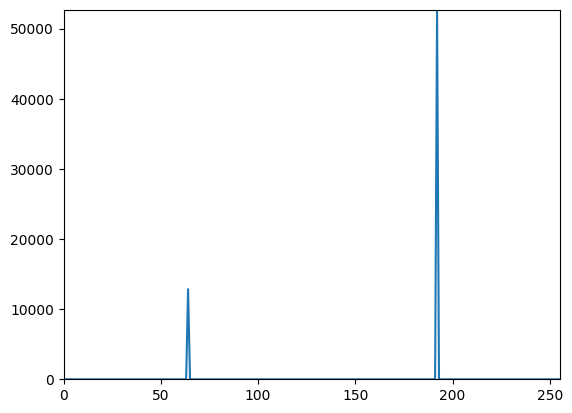
\includegraphics[width=0.45\textwidth]
{Report/Result_Images/histogram_a1.png}
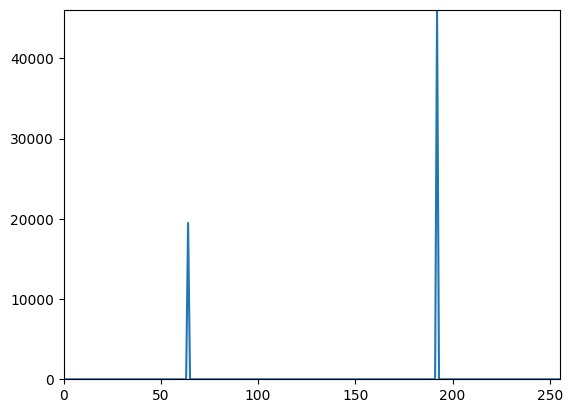
\includegraphics[width=0.45\textwidth]
{Report/Result_Images/histogram_a2.png}
\caption{The figure shows the histogram of intensities for images \emph{rect1a.tiff} and \emph{rect2a.tiff} respectively. } \label{Histogram-1a&2a}
\end{figure}

\begin{figure}[h!]
\centering
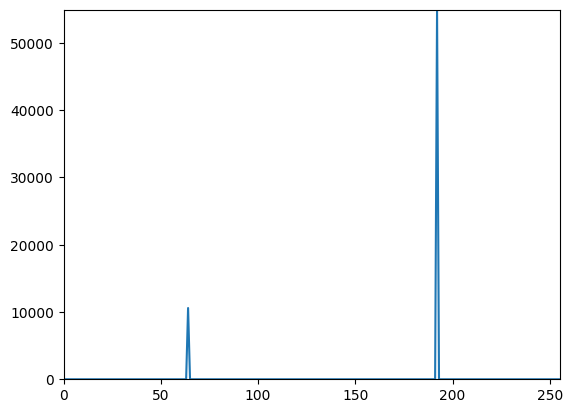
\includegraphics[width=0.45\textwidth]
{Report/Result_Images/histogram_a3.png}
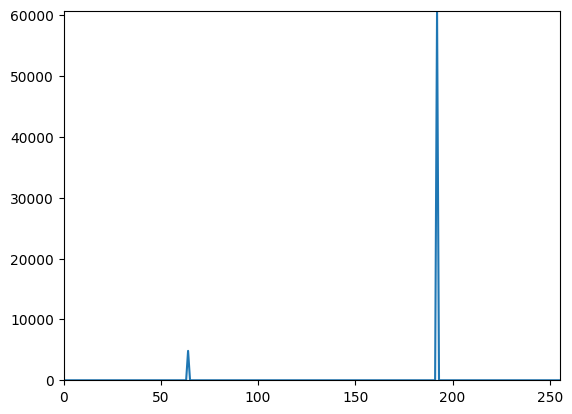
\includegraphics[width=0.45\textwidth]
{Report/Result_Images/histogram_a4.png}
\caption*{The figure shows the histogram of intensities for images \emph{rect3a.tiff} and \emph{rect4a.tiff} respectively. } \label{Histogram-3a&4a}
\end{figure}

Figures 1-4 show the histograms of intensities for image series A including {\emph{rect1a.tiff, rect2a.tiff, rect3a.tiff and rect4a.tiff}}. 
\par As the series of images are limited in their intensity distribution, the histograms are bimodal (they possess two peaks). The lower peak with lesser intensities corresponds to the foreground and the greater peak with higher intensities corresponds to the white background.

\subsection*{2. Size of Objects - Average and Standard Deviation}
In this section, we calculated the sizes or areas of the objects in each image and their standard deviations. 
The results are comprised in a table below. 
\begin{table}[h!]
\centering
\begin{tabular}{|c|c|c|c|c|}
\hline
\textbf{} & \textbf{Image 1a} & \textbf{Image 2a} & \textbf{Image 3a} & \textbf{Image 4a} \\
\hline
Obj 1 & 12848  & 3195  & 1320 &  475 \\ \hline
Obj 2 &   -         & 3285  & 1328 &  480\\ \hline
Obj 3 &    -        & 3265  & 1335 &  480\\ \hline
Obj 4 &    -        & 3248  & 1304 &  480\\ \hline
Obj 5 &    -        & 3230  & 1340 &  486\\ \hline
Obj 6 &    -        & 3262  & 1309 &  473\\ \hline
Obj 7 &    -        &  -     & 1297 &  468\\ \hline
Obj 8 &    -        &   -    & 1360 &  499\\ \hline
Obj 9 &    -        &  -     &  -    &  484\\ \hline
Obj 10 &   -         &  -     & -     &  505\\ \hline
\textbf{Average} &   12484    &  3247.5      &   1324.125    & 483  \\ \hline
\textbf{Standard Deviation} &  0      &  28.83      &    19.55   & 10.79  \\ \hline
\end{tabular}
\caption{Table of the \textbf{areas} of Images 1a, 2a, 3a and 4a, the averages and the standard deviations for each image}
\label{tab:Area-ImageSeriesA}
\end{table}
\\ The averages of the areas and the standard deviation are summarised in the last two rows. 
\subsection*{3. Perimeter of Objects - Average and Standard Deviation}
In this section, we calculated the perimeters of the objects in each image in series A and their standard deviations. 
The results are comprised in a table below. 
\begin{table}[h!]
\centering
\begin{tabular}{|c|c|c|c|c|}
\hline
\textbf{} & \textbf{Image 1a} & \textbf{Image 2a} & \textbf{Image 3a} & \textbf{Image 4a} \\
\hline
Obj 1 & 457.5 & 233.7  & 143.9 & 92.43 \\ \hline
Obj 2 &  -     & 230.1  & 148.8 & 90.98 \\ \hline
Obj 3 &  -     & 234.7  & 148.9 & 90.98 \\ \hline
Obj 4 &  -     & 236.0  & 146.9 & 92.92 \\ \hline
Obj 5 &  -     & 233.3  & 147.0 & 93.35 \\ \hline
Obj 6 &  -     & 235.1  & 147.5 & 92.05 \\ \hline
Obj 7 &  -     &   -     & 147.2 & 92.67 \\ \hline
Obj 8 &   -    &   -     & 150.5 & 93.54 \\ \hline
Obj 9 &  -     &    -    &   -    & 94.08  \\ \hline
Obj 10 & -      &  -      &   -   & 95.23  \\ \hline
\textbf{Average} &    457.5   &  233.81      &  147.59     & 92.82  \\ \hline
\textbf{Standard Deviation} &   0    &    1.88    &  1.81     & 1.25 \\ \hline
\end{tabular}
\caption{Table of the \textbf{perimeters} of Images 1a, 2a, 3a and 4a, the averages and the standard deviations for each image}
\label{tab:Perimeter-ImageSeriesA}
\end{table}
\\ The averages of the areas and the standard deviation are summarised in the last two rows. 
\newpage
\section*{Part 2.2}
In this part, we explore the relation between the square root of the mean and the coefficient of variation. 
\par Coefficient of variation is defined as the ratio of the standard deviation to the mean. It measures the rate of variability in relation to the mean.
It is expressed as 
\begin{equation*}
    cv = \frac{\sigma}{\mu'}
\end{equation*}


\subsection*{4: Graph of square root of Area against Standard Deviation}
\hl{Table 1} \ref{tab:Area-ImageSeriesA} on page \pageref{tab:Area-ImageSeriesA} contains the values for the average and standard deviation of the size (area) of the objects in the image series A. We plot these in a graph, with the X-axis being the square root of the mean and the Y-axis being the coefficient of variation. 

\begin{figure}[h!]
\centering
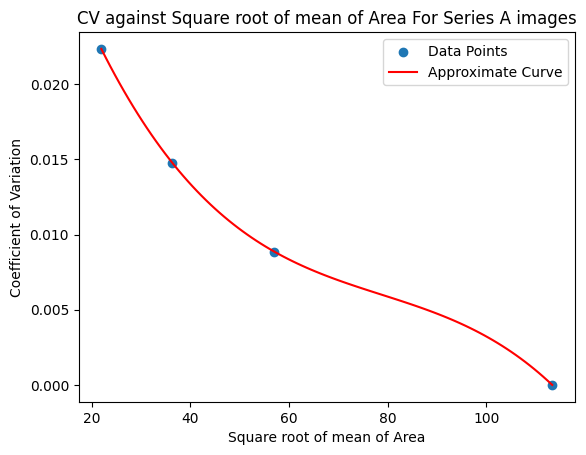
\includegraphics[width=0.9\textwidth]{Report/Result_Images/2.2_area.png}
\caption{The graph shows the relation of the area against the standard deviation, with the curve depicting the relative discretization of the area}
\label{area-relation-A}
\end{figure}

\subsection*{5: Graph of square root of Perimeter against Standard Deviation}
\hl{Table 2} \ref{tab:Perimeter-ImageSeriesA} on page \pageref{tab:Perimeter-ImageSeriesA} contains the values for the average and standard deviation of the perimeter of the objects in the image series A. We plot these in a graph, with the X-axis being the square root of the mean and the Y-axis being the coefficient of variation. 

\begin{figure}[h!]
\centering
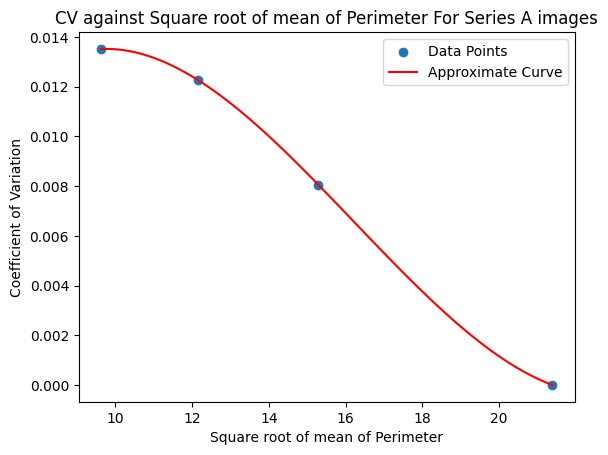
\includegraphics[width=0.9\textwidth]{Report/Result_Images/2.2_perimeter.png}
\caption{The graph shows the relation of the perimeter against the standard deviation, with the curve depicting the relative discretization of the perimeter} 
\label{perimeter-relation-A}
\end{figure}


\subsection*{6: Differences in Area and Perimeter Plot}

From figure 3 and 4 depicts the negative non-linear relationship between the square root of mean and the coefficient of variation for both area and perimeter. This downward sloping trend indicates that as the average area or perimeter increases, the coefficient of variation decreases. This is because the coefficient of variation (cv) is inversely related to the mean $\mu$: a higher mean corresponds to lower variability and vice versa. \newline
We can also see a subtle difference between the relationship between the square root of mean of area and the coefficient of variaton (as depicted by figure 2) and the relationship between  the square root of mean of perimeter and the coefficient of variaton. While both are non-negative, the slope of the graph in figure 2 begins to decrease such that a rise in the mean of area produces a smaller decline in cv. This means the effect of area on variability becomes less pronounced. This may be because as the mean area increases there comes a point where the objects reach a maximum size or density and thus further increases in average area have little effect on variability.\newline
In comparison, the slope of the graph in figure 2 begins to increase such that a rise in the mean of perimeter produces a greater decline in cv. This means the effect of perimeter on variability becomes more pronounced. This may be because as the mean perimeter increases objects begin to become more homogeneous in their shape and thus the variability decreases even more than before .
\newpage

\section*{Part 2.3}
\subsection*{7. Histograms of Series B and C images}
The following images are the histograms of intensities of image B. 
\par As we can see the images are not bi-modal like the images from series A as they do not have two pronounced peaks. We can also see that the graph is noisy, showing the high entropy of the pixel intensities.
\begin{figure}[h]
\begin{minipage}[h]{0.47\linewidth}
\begin{center}
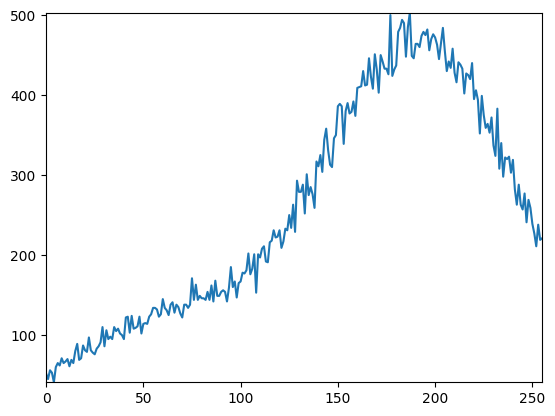
\includegraphics[width=1\linewidth]{Report/Result_Images/histogram_1b.png} 
\caption{Histogram of \emph{rect1b.tiff}}
\label{1b-histogram}
\end{center} 
\end{minipage}
\hfill
\vspace{0.2 cm}
\begin{minipage}[h]{0.47\linewidth}
\begin{center}
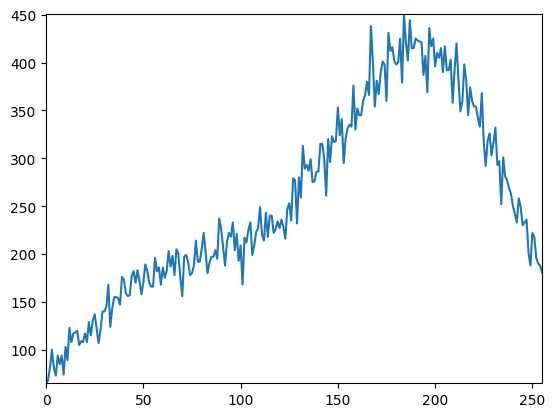
\includegraphics[width=1\linewidth]{Report/Result_Images/histogram_2b.png} 
\caption{Histogram of \emph{rect2b.tiff}}
\label{2b-Histogram}
\end{center}
\end{minipage}
\vfill
\vspace{0.2 cm}
\begin{minipage}[h]{0.47\linewidth}
\begin{center}
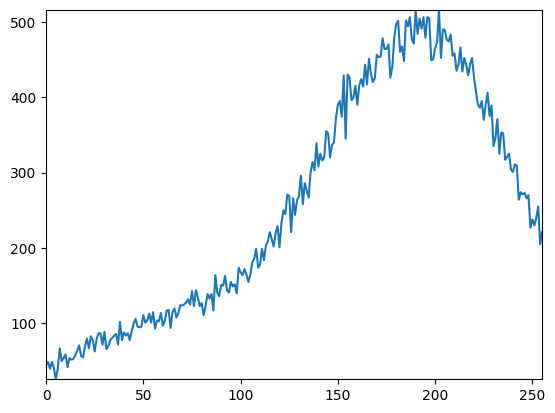
\includegraphics[width=1\linewidth]{Report/Result_Images/histogram_3b.png} 
\caption{Histogram of \emph{rect3b.tiff}}
\label{3b-Histogram}
\end{center}
\end{minipage}
\hfill
\begin{minipage}[h]{0.47\linewidth}
\begin{center}
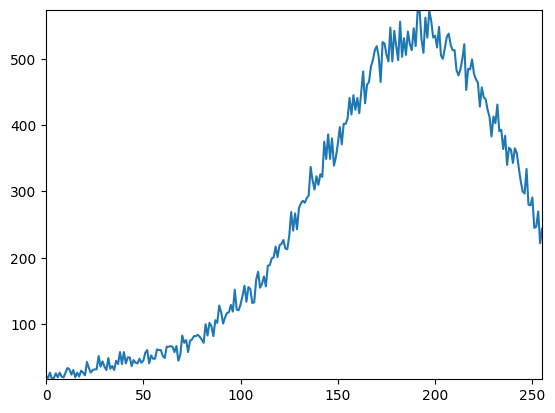
\includegraphics[width=1\linewidth]{Report/Result_Images/histogram_4b.png} 
\caption{Histogram of \emph{rect4b.tiff}}
\label{4b-Histogram}
\end{center}
\end{minipage}
\caption*{Histogram of intensities of images in series B}
\label{Histogram-B_Series}
\end{figure}

\newpage
The following images are the histograms of intensities of image C. 
\par Similar to images in series B, the images are not bi-modal like the images from series A as they do not have two pronounced peaks and have a high amount of entropy (or noise).
\begin{figure}[h!]
\begin{minipage}[h]{0.47\linewidth}
\begin{center}
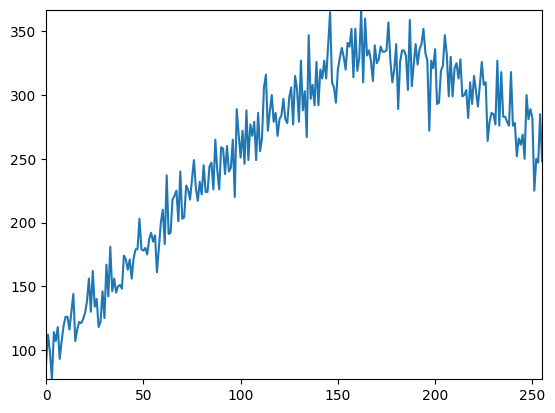
\includegraphics[width=1\linewidth]{Report/Result_Images/histogram_1c.png} 
\caption{Histogram of \emph{rect1c.tiff}}
\label{Histogram-1c}
\end{center} 
\end{minipage}
\hfill
\vspace{0.2 cm}
\begin{minipage}[h]{0.47\linewidth}
\begin{center}
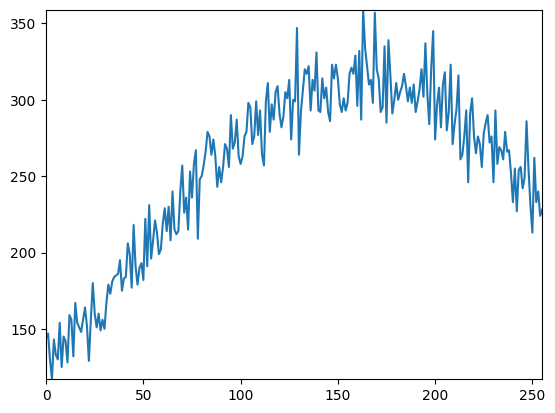
\includegraphics[width=1\linewidth]{Report/Result_Images/histogram_2c.png} 
\caption{Histogram of \emph{rect2c.tiff}}
\label{Histogram-2c}
\end{center}
\end{minipage}
\vfill
\vspace{0.2 cm}
\begin{minipage}[h]{0.47\linewidth}
\begin{center}
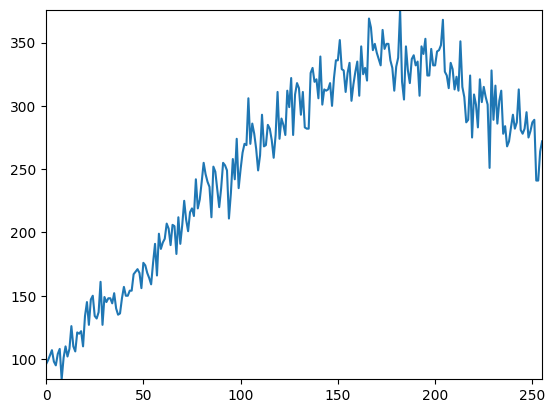
\includegraphics[width=1\linewidth]{Report/Result_Images/histogram_3c.png} 
\caption{Histogram of \emph{rect3c.tiff}}
\label{Histogram-3c}
\end{center}
\end{minipage}
\hfill
\begin{minipage}[h]{0.47\linewidth}
\begin{center}
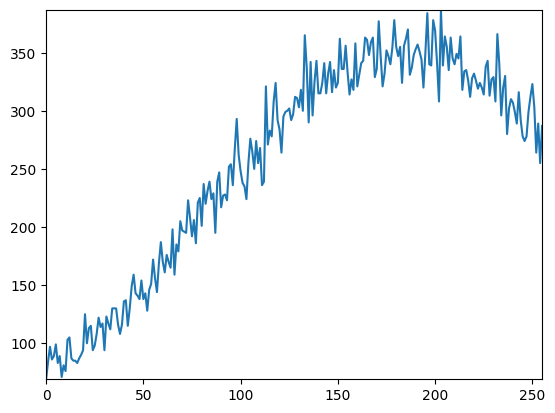
\includegraphics[width=1\linewidth]{Report/Result_Images/histogram_4c.png} 
\caption{Histogram of \emph{rect4c.tiff}}
\label{Histogram-4c}
\end{center}
\end{minipage}
\caption*{Histogram of intensities of images in series C}
\label{Histogram-C_Series}
\end{figure}

\subsection*{8. Noise Suppression with Filters and Parameters}
It is evident from figures 5 through 13 that the images from series B and C are extremely noisy and possess a high entropy. Thus, filters are needed to reduce noise levels in images. The two filters that were chosen for noise suppression were Gaussian filter and Kuwahara filter. 
% \begin{itemize}
%    \item Gaussian Filter was tested with a kernel size of 1 and 5 against noisy image series B and C. 
%    \item Kuwahara Filter was tested with a kernel size of 2 and 5 against noisy image series B and C. 
% \end{itemize}
\par The Gaussian filter is the result of blurring an image by a Gaussian function and is named after mathematician and scientist Carl Friedrich Gauss. The formula of the Gaussian filter can be given by 
\begin{equation*}
    G(x) = \frac{1}{\sqrt{2\pi\sigma^2}} e^{-\frac{x^2}{2\sigma^2}}
\end{equation*}

For this paper we applied the Gaussian filter on these series of images with two different kernel sizes: 1 and 5.
\subsubsection*{Gaussian Filter with a Kernel Size of 1}


\paragraph*{\textbf{Series B}}
Figures \ref{hb1-Gaussian and Kernel 1},  \ref{hb2-Gaussian and Kernel 1}, \ref{hb3-Gaussian and Kernel 1}, \ref{hb4-Gaussian and Kernel 1} are the resulting images after a Gaussian filter with a kernel size of 1 was used to suppress the noise in image series B. 
\begin{figure}[h!]
\begin{minipage}[h]{0.47\linewidth}
\begin{center}
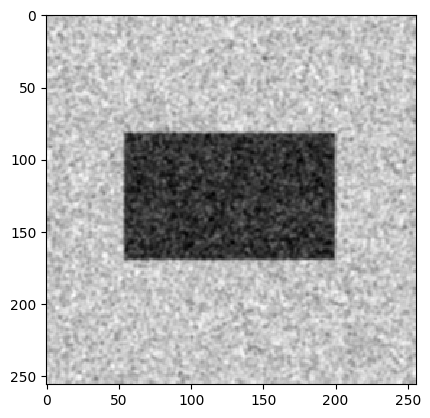
\includegraphics[width=1\linewidth]{Report/Result_Images/image_hb1.png} 
\caption{\emph{rect1b.tif} after}
\label{hb1-Gaussian and Kernel 1}
\end{center} 
\end{minipage}
\hfill
\vspace{0.2 cm}
\begin{minipage}[h]{0.47\linewidth}
\begin{center}
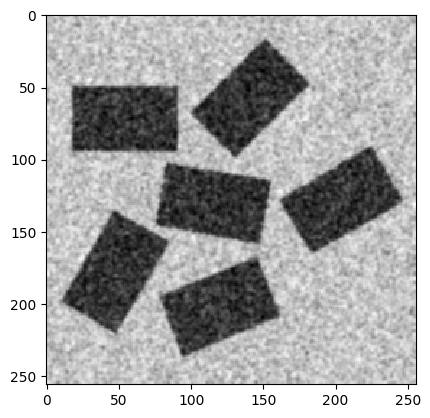
\includegraphics[width=1\linewidth]{Report/Result_Images/image_hb2.png} 
\caption{\emph{rect2b.tif} after}
\label{hb2-Gaussian and Kernel 1}
\end{center}
\end{minipage}
\vfill
\vspace{0.2 cm}
\begin{minipage}[h]{0.47\linewidth}
\begin{center}
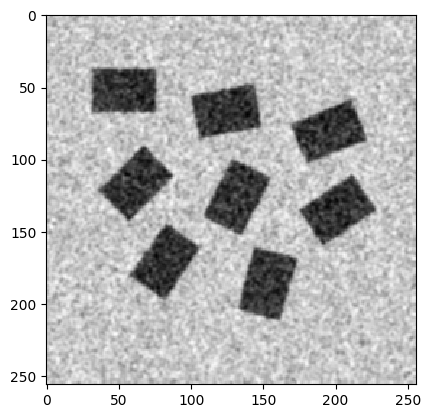
\includegraphics[width=1\linewidth]{Report/Result_Images/image_hb3.png} 
\caption{\emph{rect3b.tif} after}
\label{hb3-Gaussian and Kernel 1}
\end{center}
\end{minipage}
\hfill
\begin{minipage}[h]{0.47\linewidth}
\begin{center}
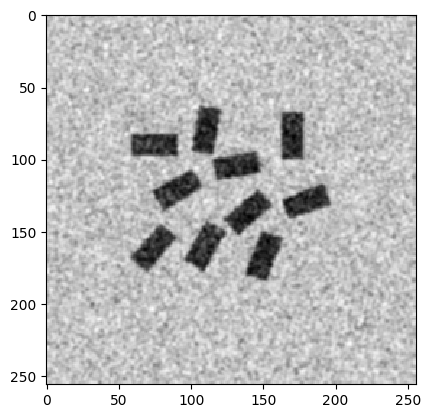
\includegraphics[width=1\linewidth]{Report/Result_Images/image_hb4.png} 
\caption{\emph{rect4b.tif} after}
\label{hb4-Gaussian and Kernel 1}
\end{center}
\end{minipage}
\caption*{Gaussian Filter with kernel size 1 has been applied to Image Series B}
\label{hb1-4 Gaussian1}
\end{figure}

A comparison of the original B series images and the images presented in figures 12 to 15 show the blurring effect of the Gaussian filter on images with noise. 


\newpage
\paragraph*{\textbf{Series C}}
Figures \ref{hc1-Gaussian and Kernel 1}, \ref{hc2-Gaussian and Kernel 1}, \ref{hc3-Gaussian and Kernel 1} and \ref{hc4-Gaussian and Kernel 1} are the resulting images after a Gaussian filter with a kernel size of 1 was used to suppress the noise in image series C. 
\begin{figure}[h!]
\begin{minipage}[h]{0.47\linewidth}
\begin{center}
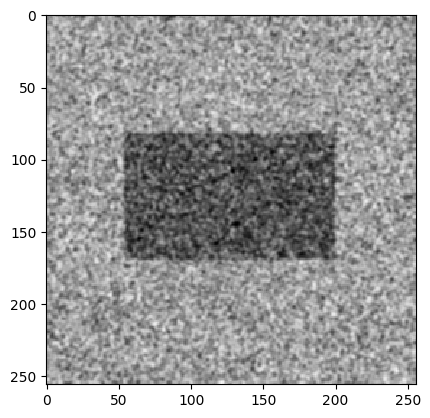
\includegraphics[width=1\linewidth]{Report/Result_Images/image_hc1.png} 
\caption{\emph{rect1c.tif} after}
\label{hc1-Gaussian and Kernel 1}
\end{center} 
\end{minipage}
\hfill
\vspace{0.2 cm}
\begin{minipage}[h]{0.47\linewidth}
\begin{center}
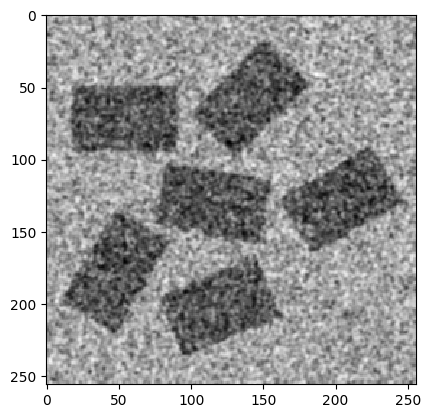
\includegraphics[width=1\linewidth]{Report/Result_Images/image_hc2.png} 
\caption{\emph{rect2c.tif} after}
\label{hc2-Gaussian and Kernel 1}
\end{center}
\end{minipage}
\vfill
\vspace{0.2 cm}
\begin{minipage}[h]{0.47\linewidth}
\begin{center}
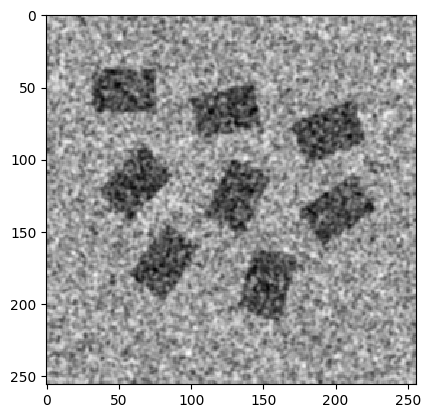
\includegraphics[width=1\linewidth]{Report/Result_Images/image_hc3.png} 
\caption{\emph{rect3c.tif} after}
\label{hc3-Gaussian and Kernel 1}
\end{center}
\end{minipage}
\hfill
\begin{minipage}[h]{0.47\linewidth}
\begin{center}
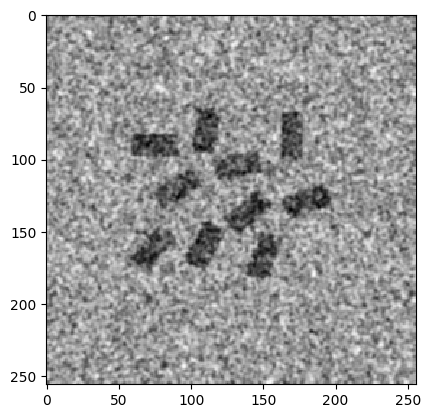
\includegraphics[width=1\linewidth]{Report/Result_Images/image_hc4.png} 
\caption{\emph{rect4c.tif} after}
\label{hc4-Gaussian and Kernel 1}
\end{center}
\end{minipage}
\caption*{Gaussian Filter with kernel size 1 has been applied to Image Series C}
\label{hc1-4 Gaussian1}
\end{figure}

A comparison of the original C series images and the images presented in figures 16 to 19 show the blurring effect of the Gaussian filter on images with noise. 

\newpage
\subsubsection*{Gaussian Filter with a Kernel Size of 5}
\paragraph*{\textbf{Series B}}
Figures \ref{hb5-Gaussian and Kernel 5}, \ref{hb6-Gaussian and Kernel 5}, \ref{hb7-Gaussian and Kernel 5} and \ref{hb8-Gaussian and Kernel 5} are the resulting images after a Gaussian filter with a kernel size of 5 was used to suppress the noise in image series B. 
\begin{figure}[h!]
\begin{minipage}[h]{0.47\linewidth}
\begin{center}
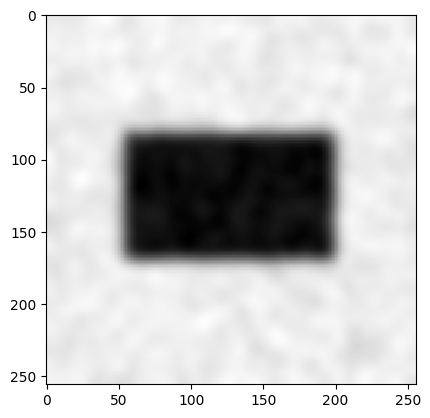
\includegraphics[width=1\linewidth]{Report/Result_Images/image_hb5.png} 
\caption{\emph{rect1b.tif} after}
\label{hb5-Gaussian and Kernel 5}
\end{center} 
\end{minipage}
\hfill
\vspace{0.2 cm}
\begin{minipage}[h]{0.47\linewidth}
\begin{center}
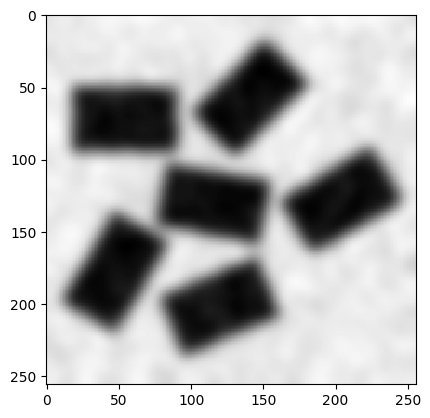
\includegraphics[width=1\linewidth]{Report/Result_Images/image_hb6.png} 
\caption{\emph{rect2b.tif} after}
\label{hb6-Gaussian and Kernel 5}
\end{center}
\end{minipage}
\vfill
\vspace{0.2 cm}
\begin{minipage}[h]{0.47\linewidth}
\begin{center}
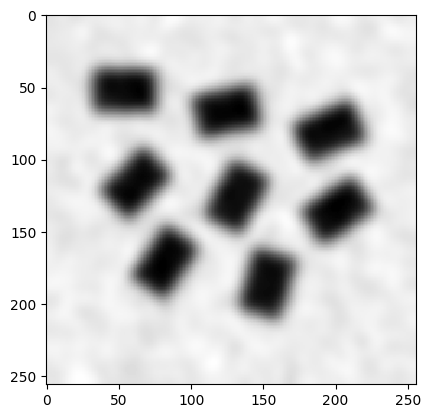
\includegraphics[width=1\linewidth]{Report/Result_Images/image_hb7.png} 
\caption{\emph{rect3b.tif} after}
\label{hb7-Gaussian and Kernel 5}
\end{center}
\end{minipage}
\hfill
\begin{minipage}[h]{0.47\linewidth}
\begin{center}
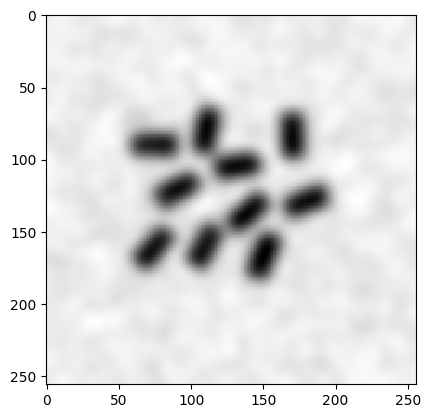
\includegraphics[width=1\linewidth]{Report/Result_Images/image_hb8.png} 
\caption{\emph{rect4b.tif} after}
\label{hb8-Gaussian and Kernel 5}
\end{center}
\end{minipage}
\caption*{Gaussian Filter with kernel size 5 has been applied to Image Series B}
\label{hb5-8 Gaussian5}
\end{figure}


\newpage
\paragraph*{\textbf{Series C}}
Figures \ref{hc5-Gaussian and Kernel 5}, \ref{hc6-Gaussian and Kernel 5}, \ref{hc7-Gaussian and Kernel 5} and \ref{hc8-Gaussian and Kernel 5} are the resulting images after a Gaussian filter with a kernel size of 5 was used to suppress the noise in image series C. 
\begin{figure}[h!]
\begin{minipage}[h]{0.5\linewidth}
\begin{center}
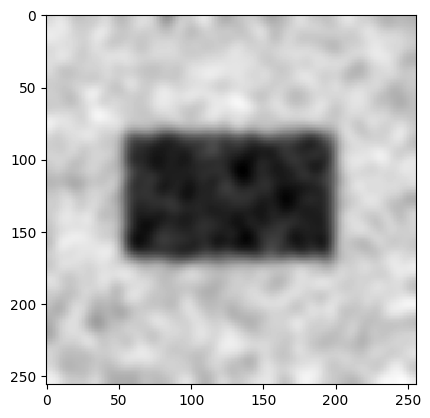
\includegraphics[width=1\linewidth]{Report/Result_Images/image_hc5.png} 
\caption{\emph{rect1c.tif} after}
\label{hc5-Gaussian and Kernel 5}
\end{center} 
\end{minipage}
\hfill
\vspace{0.2 cm}
\begin{minipage}[h]{0.47\linewidth}
\begin{center}
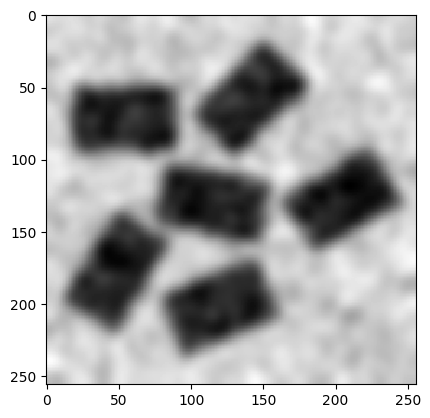
\includegraphics[width=1\linewidth]{Report/Result_Images/image_hc6.png} 
\caption{\emph{rect2c.tif} after}
\label{hc6-Gaussian and Kernel 5}
\end{center}
\end{minipage}
\vfill
\vspace{0.2 cm}
\begin{minipage}[h]{0.47\linewidth}
\begin{center}
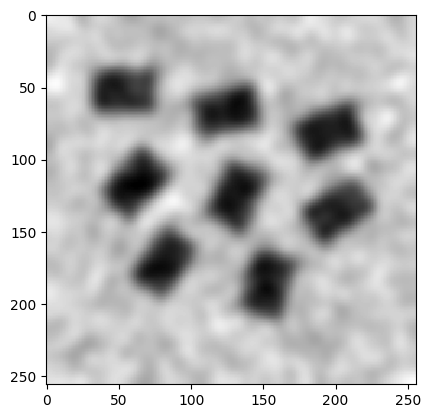
\includegraphics[width=1\linewidth]{Report/Result_Images/image_hc7.png} 
\caption{\emph{rect3c.tif} after}
\label{hc7-Gaussian and Kernel 5}
\end{center}
\end{minipage}
\hfill
\begin{minipage}[h]{0.47\linewidth}
\begin{center}
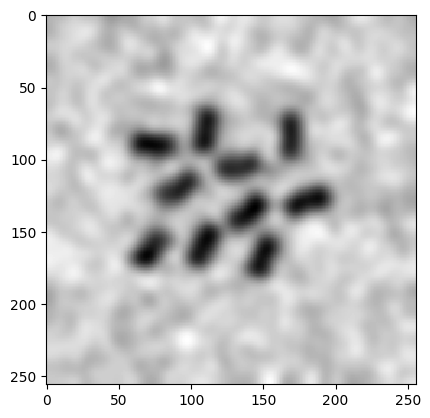
\includegraphics[width=1\linewidth]{Report/Result_Images/image_hc8.png} 
\caption{\emph{rect4c.tif} after}
\label{hc8-Gaussian and Kernel 5}
\end{center}
\end{minipage}
\caption*{Gaussian Filter with kernel size 5 has been applied to Image Series C}
\label{hc5-8 Gaussian5}
\end{figure}

As seen in figures 20 to 27, with a kernel of size 5 the blurring effect is larger as a larger neighborhood of surrounding pixels is used to get the average, reducing the variation in pixel intensities even more.  

~\\ Another filter that can be used to suppress the noise in image series B and C, is Kuwahara Filter. 
\par Kuwahara Filter is a non-linear edge-preserving filter. This means that it smooths out the image without disturbing the sharpness and positions of the edges. It does this by dividing the image into four quadrants and calculating the average value and variance (standard deviation) per compass region.
~\\ Average of the region is denoted as $(i)$ where  $\sigma_i$= min ${{\sigma_j}}_{1..4}$
The kernels can be square, rectangular or elliptical. While larger kernels tend to smooth the image intensities more, they often erode image details. Thus small kernel sizes are more suitable for our study as they smooth while preserving image detail. Thus, kernel sizes of 2 and 5 were chosen. 


\subsubsection*{Kuwahara Filter with a Kernel Size of 2}
\paragraph*{\textbf{Series B}}
Figures \ref{kb1-Kuwahara and Kernel 2}, \ref{kb2-Kuwahara and Kernel 2}, \ref{kb3-Kuwahara and Kernel 2} and \ref{kb4-Kuwahara and Kernel 2} are the resulting images after a Kuwahara filter with a kernel size of 2 was used to suppress the noise in image series B. 
\begin{figure}[h!]
\begin{minipage}[h]{0.47\linewidth}
\begin{center}
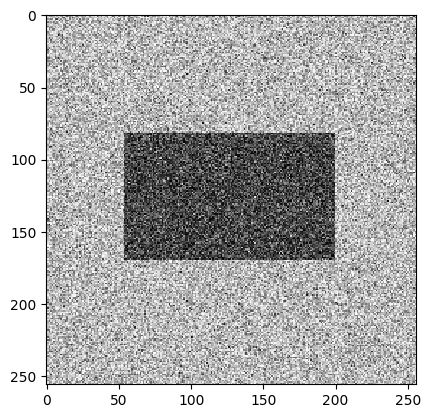
\includegraphics[width=1\linewidth]{Report/Result_Images/image_kb1.png} 
\caption{\emph{rect1b.tif} after}
\label{kb1-Kuwahara and Kernel 2}
\end{center} 
\end{minipage}
\hfill
\vspace{0.2 cm}
\begin{minipage}[h]{0.47\linewidth}
\begin{center}
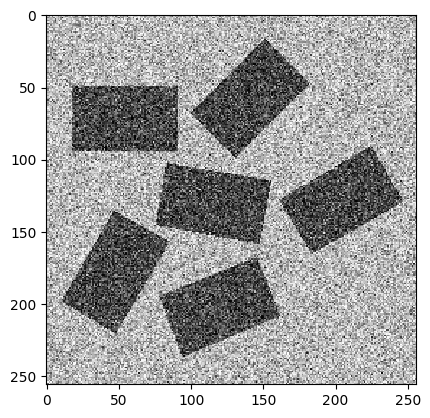
\includegraphics[width=1\linewidth]{Report/Result_Images/image_kb2.png} 
\caption{\emph{rect2b.tif} after}
\label{kb2-Kuwahara and Kernel 2}
\end{center}
\end{minipage}
\vfill
\vspace{0.2 cm}
\begin{minipage}[h]{0.47\linewidth}
\begin{center}
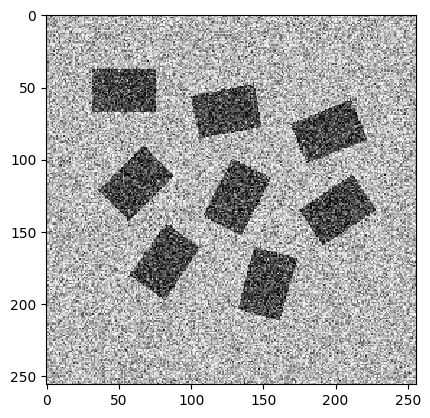
\includegraphics[width=1\linewidth]{Report/Result_Images/image_kb3.png} 
\caption{\emph{rect3b.tif} after}
\label{kb3-Kuwahara and Kernel 2}
\end{center}
\end{minipage}
\hfill
\begin{minipage}[h]{0.47\linewidth}
\begin{center}
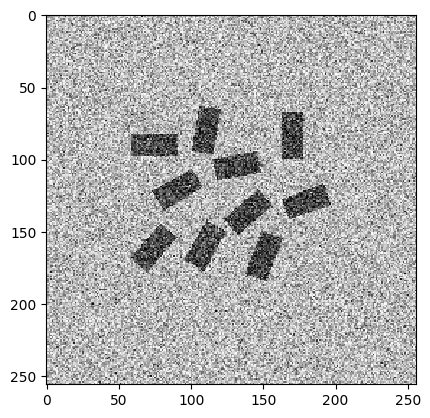
\includegraphics[width=1\linewidth]{Report/Result_Images/image_kb4.png} 
\caption{\emph{rect4b.tif} after}
\label{kb4-Kuwahara and Kernel 2}
\end{center}
\end{minipage}
\caption*{Kuwahara Filter with kernel size 2 has been applied to Image Series B}
\label{kb1-4 Kuwahara2}
\end{figure}
 
\paragraph*{\textbf{Series C}}
Figures \ref{kc1-Kuwahara and Kernel 2}, \ref{kc2-Kuwahara and Kernel 2}, \ref{kc3-Kuwahara and Kernel 2} and \ref{kc4-Kuwahara and Kernel 2} are the resulting images after a Kuwahara filter with a kernel size of 2 was used to suppress the noise in image series C. 
\begin{figure}[h!]
\begin{minipage}[h]{0.47\linewidth}
\begin{center}
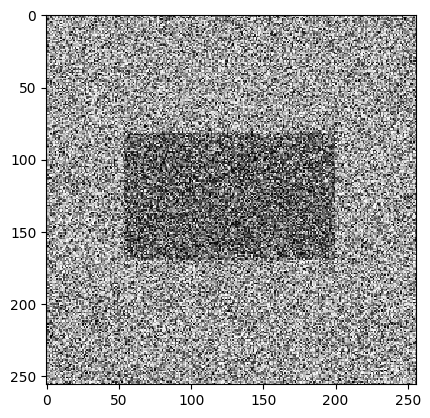
\includegraphics[width=1\linewidth]{Report/Result_Images/image_kc1.png} 
\caption{\emph{rect1c.tif} after}
\label{kc1-Kuwahara and Kernel 2}
\end{center} 
\end{minipage}
\hfill
\vspace{0.2 cm}
\begin{minipage}[h]{0.47\linewidth}
\begin{center}
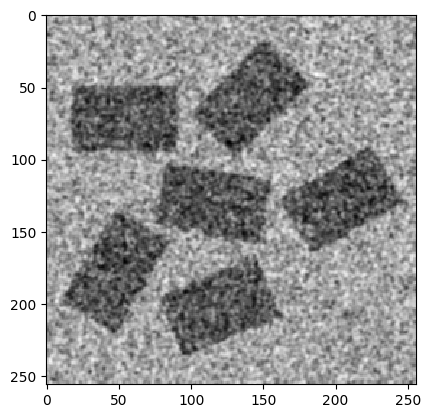
\includegraphics[width=1\linewidth]{Report/Result_Images/image_hc2.png} 
\caption{\emph{rect2c.tif} after}
\label{kc2-Kuwahara and Kernel 2}
\end{center}
\end{minipage}
\vfill
\vspace{0.2 cm}
\begin{minipage}[h]{0.47\linewidth}
\begin{center}
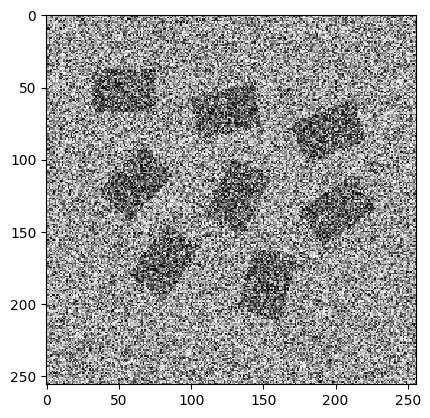
\includegraphics[width=1\linewidth]{Report/Result_Images/image_kc3.png} 
\caption{\emph{rect3c.tif} after}
\label{kc3-Kuwahara and Kernel 2}
\end{center}
\end{minipage}
\hfill
\begin{minipage}[h]{0.47\linewidth}
\begin{center}
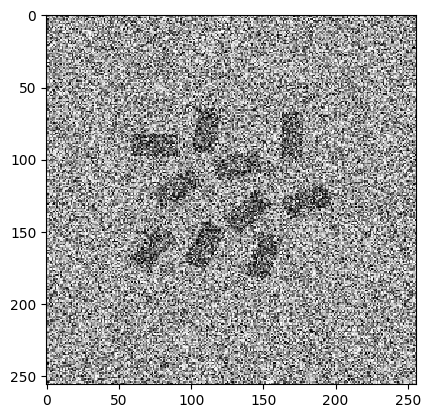
\includegraphics[width=1\linewidth]{Report/Result_Images/image_kc4.png} 
\caption{\emph{rect4c.tif} after}
\label{kc4-Kuwahara and Kernel 2}
\end{center}
\end{minipage}
\caption*{Kuwahara Filter with kernel size 2 has been applied to Image Series C}
\label{kc1-4 Kuwahara2}
\end{figure}

A comparison of the original B and C series images and the images presented in figures 28 to 35 show the blurring effect of the Kuwahara filter on images with noise.


\newpage
\subsubsection*{Kuwahara Filter with a Kernel Size of 5}
\paragraph*{\textbf{Series B}}
Figures \ref{kb5-Kuwahara and Kernel 5}, \ref{kb6-Kuwahara and Kernel 5}, \ref{kb7-Kuwahara and Kernel 5} and \ref{kb8-Kuwahara and Kernel 5} are the resulting images after a Kuwahara filter with a kernel size of 5 was used to suppress the noise in image series B. 
\begin{figure}[h!]
\begin{minipage}[h]{0.47\linewidth}
\begin{center}
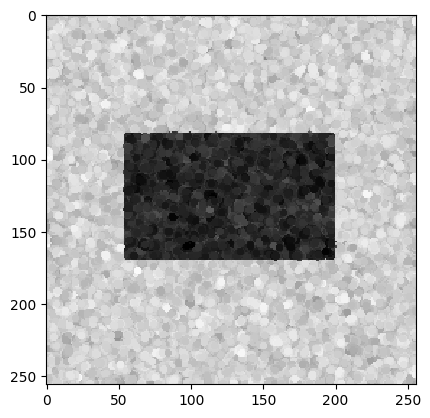
\includegraphics[width=1\linewidth]{Report/Result_Images/image_kb5.png} 
\caption{\emph{rect1b.tif} after}
\label{kb5-Kuwahara and Kernel 5}
\end{center} 
\end{minipage}
\hfill
\vspace{0.2 cm}
\begin{minipage}[h]{0.47\linewidth}
\begin{center}
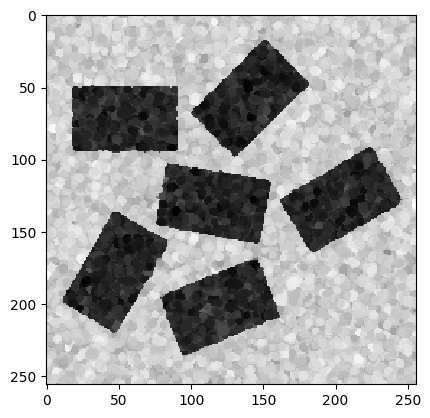
\includegraphics[width=1\linewidth]{Report/Result_Images/image_kb6.png} 
\caption{\emph{rect2b.tif} after}
\label{kb6-Kuwahara and Kernel 5}
\end{center}
\end{minipage}
\vfill
\vspace{0.2 cm}
\begin{minipage}[h]{0.47\linewidth}
\begin{center}
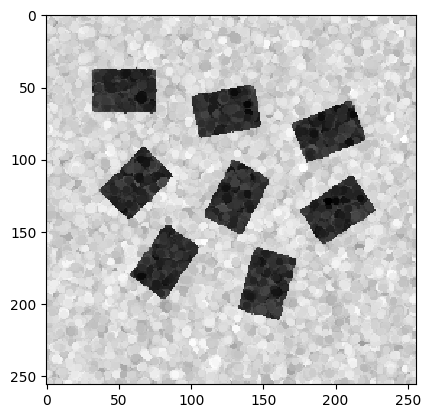
\includegraphics[width=1\linewidth]{Report/Result_Images/image_kb7.png} 
\caption{\emph{rect3b.tif} after}
\label{kb7-Kuwahara and Kernel 5}
\end{center}
\end{minipage}
\hfill
\begin{minipage}[h]{0.47\linewidth}
\begin{center}
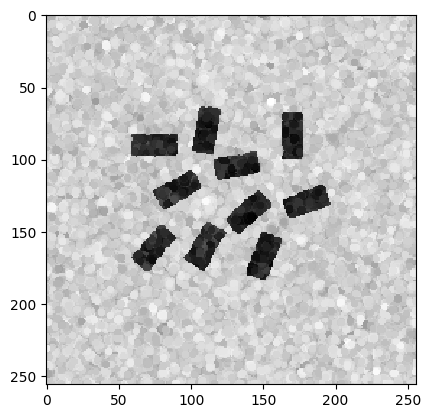
\includegraphics[width=1\linewidth]{Report/Result_Images/image_kb8.png} 
\caption{\emph{rect4b.tif} after}
\label{kb8-Kuwahara and Kernel 5}
\end{center}
\end{minipage}
\caption*{Kuwahara Filter with kernel size 5 has been applied to Image Series B}
\label{kb5-8 Kuwahara5}
\end{figure}
\newpage
\paragraph*{\textbf{Series C}}
Figures \ref{kc5-Kuwahara and Kernel 5}, \ref{kc6-Kuwahara and Kernel 5},  \ref{kc7-Kuwahara and Kernel 5} and \ref{kc8-Kuwahara and Kernel 5} are the resulting images after a Kuwahara filter with a kernel size of 5 was used to suppress the noise in image series C. 
\begin{figure}[h!]
\begin{minipage}[h]{0.47\linewidth}
\begin{center}
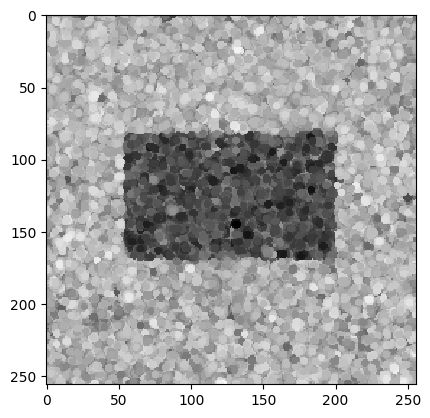
\includegraphics[width=1\linewidth]{Report/Result_Images/image_kc5.png} 
\caption{\emph{rect1c.tif} after}
\label{kc5-Kuwahara and Kernel 5}
\end{center} 
\end{minipage}
\hfill
\vspace{0.2 cm}
\begin{minipage}[h]{0.47\linewidth}
\begin{center}
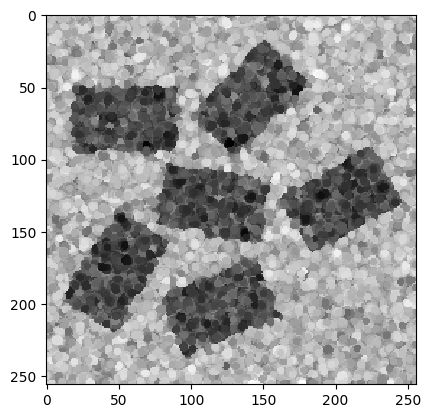
\includegraphics[width=1\linewidth]{Report/Result_Images/image_kc6.png} 
\caption{\emph{rect2c.tif} after}
\label{kc6-Kuwahara and Kernel 5}
\end{center}
\end{minipage}
\vfill
\vspace{0.2 cm}
\begin{minipage}[h]{0.47\linewidth}
\begin{center}
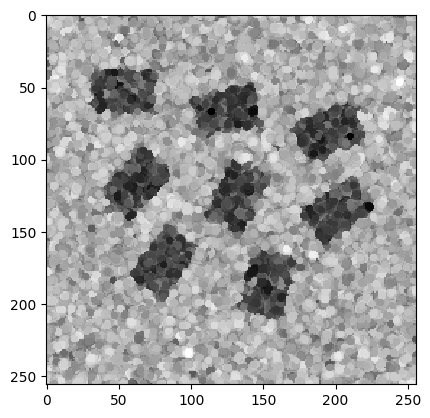
\includegraphics[width=1\linewidth]{Report/Result_Images/image_kc7.png} 
\caption{\emph{rect3c.tif} after}
\label{kc7-Kuwahara and Kernel 5}
\end{center}
\end{minipage}
\hfill
\begin{minipage}[h]{0.47\linewidth}
\begin{center}
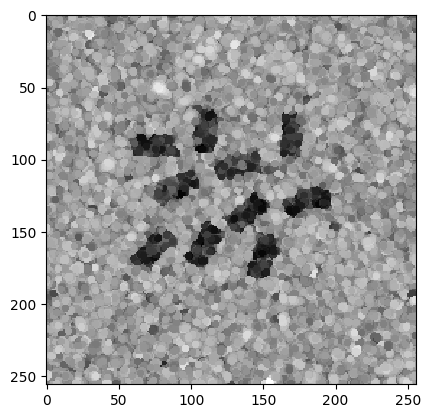
\includegraphics[width=1\linewidth]{Report/Result_Images/image_kc8.png} 
\caption{\emph{rect4c.tif} after}
\label{kc8-Kuwahara and Kernel 5}
\end{center}
\end{minipage}
\caption*{Kuwahara Filter with kernel size 5 has been applied to Image Series C}
\label{kc5-8 Kuwahara5}
\end{figure}

A larger kernel size produces greater blurring as a larger neighborhood of pixels is used to compute the value of the central pixel, leading to less variation in pixel intensities. 
\newpage

\subsection*{9. Area and Perimeter Calculation for the Noisy Images}
\par In this section we calculated the sizes or areas of objects in each image in series B and C and their standard deviations. 
\par Tables \ref{tab:Area-Series B} and \ref{tab:Perimeter-Series B} contain the of the area and perimeter of the objects in series B and their average and standard deviations. 

\begin{table}[h!]
\centering
\begin{tabular}{|c|c|c|c|c|}
\hline
\textbf{} & \textbf{Image 1b} & \textbf{Image 2b} & \textbf{Image 3b} & \textbf{Image 4b} \\
\hline
Obj 1 & 9493      & 2399  & 987 &  368 \\ \hline
Obj 2 &    -        & 2399  & 998 &  359\\ \hline
Obj 3 &   -         & 2410  & 997 &  355\\ \hline
Obj 4 &   -         & 2435  & 964 &  369\\ \hline
Obj 5 &   -         & 2396  & 977 &  349\\ \hline
Obj 6 &   -         & 2349  & 991 &  352\\ \hline
Obj 7 &    -        &   -    & 978 &  365\\ \hline
Obj 8 &   -         &   -    & 990 &  342 \\ \hline
Obj 9 &    -        &   -    &  -    & 342\\ \hline
Obj 10 &   -         &   -   &  -    & 384\\ \hline
\textbf{Average} &   9493    &  2398      &   985.3   & 358.5  \\ \hline
\textbf{Standard Deviation} &  0      &  25.6      &    10.8   & 12.6  \\ \hline
\end{tabular}
\caption{Table of the areas of Images 1b, 2b, 3b and 4b.}
\label{tab:Area-Series B}
\end{table}

\begin{table}[h!]
\centering
\begin{tabular}{|c|c|c|c|c|}
\hline
\textbf{} & \textbf{Image 1b} & \textbf{Image 2b} & \textbf{Image 3b} & \textbf{Image 4b} \\
\hline
Obj 1 & 571.8      & 331.1  & 216.1 &  124 \\ \hline
Obj 2 &  -          & 318.6  & 206.4 &  116.8\\ \hline
Obj 3 & -           & 309.9  & 211.5 &  110.8\\ \hline
Obj 4 & -           & 350.6  & 179.7 &  127.6\\ \hline
Obj 5 &  -          & 311.0  & 213 &  124.8\\ \hline
Obj 6 &  -          & 350.9  & 195.4 &  110.2\\ \hline
Obj 7 &  -          &    -   & 201 &  115\\ \hline
Obj 8 &  -          &   -    & 192 &  132.6 \\ \hline
Obj 9 &  -          &   -    &  -    & 119.8\\ \hline
Obj 10 &  -          &   -    & -     & 134.3\\ \hline
\textbf{Average} &   571.8    &  328.7      &   201.9   & 121.6 \\ \hline
\textbf{Standard Deviation} &  0      &  17.1     &   11.5   & 8  \\ \hline
\end{tabular}
\caption{Table of the perimeter of Images 1b, 2b, 3b and 4b.}
\label{tab:Perimeter-Series B}
\end{table}

\newpage
\par Tables \ref{tab:Area-Series C} and \ref{tab:Perimeter-Series C} contain the areas and perimeters of the objects in series C along with their average and standard deviations. 
\begin{table}[h!]
\centering
\begin{tabular}{|c|c|c|c|c|}
\hline
\textbf{} & \textbf{Image 1c} & \textbf{Image 2c} & \textbf{Image 3c} & \textbf{Image 4c} \\
\hline
Obj 1 & 6974     & 1779     & 717 &  291 \\ \hline
Obj 2 &    -        & 1804  & 797 &  277\\ \hline
Obj 3 &   -         & 1882  & 797 &  291\\ \hline
Obj 4 &   -         & 1844  & 804 &  152\\ \hline
Obj 5 &   -         & 1827  & 786 &  115\\ \hline
Obj 6 &   -         & 1830  & 51  &  226\\ \hline
Obj 7 &    -        &   44  & 765 &  294\\ \hline
Obj 8 &   -         &   -   & 692 &  601 \\ \hline
Obj 9 &    -        &  -    & 771 &  330\\ \hline
Obj 10 &   -         &  -   &  72   & 255\\ \hline
\end{tabular}
\caption{Table of the areas of Images 1c, 2c, 3c and 4c.}
\label{tab:Area-Series C}
\end{table}

\begin{table}[h!]
\centering
\begin{tabular}{|c|c|c|c|c|}
\hline
\textbf{} & \textbf{Image 1c} & \textbf{Image 2c} & \textbf{Image 3c} & \textbf{Image 4c} \\
\hline
Obj 1 & 1526  & 758.3   & 493.1 &  268.9 \\ \hline
Obj 2 &    -  & 528.9  & 423.9 &  325.3 \\ \hline
Obj 3 &   -   & 743.7  & 406.7 &  232.5\\ \hline
Obj 4 &   -   & 763.2  & 505.5 &  172.9 \\ \hline
Obj 5 &   -   & 754.1  & 564.1 &  176.6 \\ \hline
Obj 6 &   -   & 842.8  & 90.75  &  248.5 \\ \hline
Obj 7 &    -  & 84.07  & 533.8 &  197.1 \\ \hline
Obj 8 &   -   &   -   & 442.0 &  442.1 \\ \hline
Obj 9 &    -  &  -    & 541.4  &  194.6\\ \hline
Obj 10 &   -  &  -   & 79.65  & 262.2 \\ \hline
\end{tabular}
\caption{Table of the Perimeter of Images 1c, 2c, 3c and 4c.}
\label{tab:Perimeter-Series C}
\end{table}
\newpage
Tables \ref{tab:Area-SeriesB-Gaussian1} and \ref{tab:Perimeter-SeriesB-Gaussian1} contain of the areas and perimeters of the objects in series B after a Gaussian filter with a kernel of size 1 is applied and their average and standard deviations.

\begin{table}[h!]
\centering
\begin{tabular}{|c|c|c|c|c|}
\hline
\textbf{} & \textbf{Image 1b} & \textbf{Image 2b} & \textbf{Image 3b} & \textbf{Image 4b} \\
\hline
Obj 1 & 12340      & 3008  & 1199 &  403 \\ \hline
Obj 2 &   -         & 3019  & 1214 &  408\\ \hline
Obj 3 &   -         & 3042  & 1188 &  387\\ \hline
Obj 4 &   -         & 3038  & 1164 &  402\\ \hline
Obj 5 &   -        & 3014  & 1210 &  397\\ \hline
Obj 6 &    -        & 3004  & 1197 &  402\\ \hline
Obj 7 &   -         &  -     & 1171 &  404\\ \hline
Obj 8 &    -        &  -     & 1244 &  406 \\ \hline
Obj 9 &   -         & -      &  -    &  392\\ \hline
Obj 10 &  -         &  -     &  -    &  439\\ \hline
\textbf{Average} &   12340    &  3020.33      &   1198.38    & 404  \\ \hline
\textbf{Standard Deviation} &  0      &  14.38      &    23.72   & 13.18  \\ \hline
\end{tabular}
\caption{Table of the areas of Images 1b, 2b, 3b and 4b after a Gaussian filter with kernel = 1 is applied }
\label{tab:Area-SeriesB-Gaussian1}
\end{table}


\begin{table}[h!]
\centering
\begin{tabular}{|c|c|c|c|c|}
\hline
\textbf{} & \textbf{Image 1b} & \textbf{Image 2b} & \textbf{Image 3b} & \textbf{Image 4b} \\
\hline
Obj 1 & 482.58     & 236.1 & 151.7 &  87.83 \\ \hline
Obj 2 &            & 245.8  & 145 &  89.30\\ \hline
Obj 3 &            & 237.7  & 148.7 &  91.17\\ \hline
Obj 4 &            & 243.8  & 146.9 &  87.76\\ \hline
Obj 5 &            & 243.5  & 144.8 &  87.56\\ \hline
Obj 6 &            & 244.1  & 144.9 &  86.87\\ \hline
Obj 7 &            &       & 144.8 &  86.54\\ \hline
Obj 8 &            &       & 145.2 &  93.57 \\ \hline
Obj 9 &            &       &      &  86.76\\ \hline
Obj 10 &           &       &      &  90.53\\ \hline
\textbf{Average} &   482.58    &  241.82      &   146.5    & 88.98  \\ \hline
\textbf{Standard Deviation} &  0      &  3.59       &    2.34   & 2.06  \\ \hline
\end{tabular}
\caption{Table of the perimeters of Images 1b, 2b, 3b and 4b after a Gaussian filter with kernel = 1 is applied }
\label{tab:Perimeter-SeriesB-Gaussian1}
\end{table}

\newpage 
Tables \ref{tab:Area-SeriesC-Gaussian1} and \ref{tab:Perimeter-SeriesC-Gaussian1} contain areas and perimeters of the objects in series C after a Gaussian filter with a kernel of size 1 is applied along with their average and standard deviations.

\begin{table}[h!]
\centering
\begin{tabular}{|c|c|c|c|c|}
\hline
\textbf{} & \textbf{Image 1c} & \textbf{Image 2c} & \textbf{Image 3c} & \textbf{Image 4c} \\
\hline
Obj 1 & 4239   & 839 & 404 &  82 \\ \hline
Obj 2 &  307   & 212  & 57 &  60\\ \hline
Obj 3 &  47    & 101  & 480 &  125\\ \hline
Obj 4 &  84    & 1270  & 49 &  214\\ \hline
Obj 5 &  60    & 41   & 421 &  111\\ \hline
Obj 6 &   76   &  53  & 70 &  50\\ \hline
Obj 7 &  559   &  42     & 88 &  59\\ \hline
Obj 8 &   249  &   159  & 471 &  242 \\ \hline
Obj 9 &  93    &    194   &   528   &  206\\ \hline
Obj 10 & 43    &     1304  &   410  &  165\\ \hline
Obj 11 &  -     &   1392   &   61 &  203\\ \hline
Obj 12 &  -  &     44  &      131  &  243\\ \hline
Obj 13 &  -     &  69   &    71  &  90\\ \hline
Obj 14 &  -  &     56 &    389  &   -\\ \hline
Obj 15 &  -   &    56   &   405   & -  \\ \hline
Obj 16 &  -   &    45 &     90 &   - \\ \hline
Obj 17 &  -    &   208   &   73   & - \\ \hline
Obj 18 &  -   &    639  &    -  &  - \\ \hline
Obj 19 &  -     &    108   &   -   &  \\ \hline
Obj 20 &  - &     93  &  -    & - \\ \hline
Obj 21 &  -     &   253   &    -  &  \\ \hline
Obj 22 & -   &     68  &   -   & - \\ \hline
Obj 23 &  -  &    51   &  -    & - \\ \hline
Obj 24 &  -  &     482  & -     & - \\ \hline
Obj 25 &  -     &  188   &  -    & -  \\ \hline
Obj 26 &  -  &     274  &  -    & - \\ \hline
Obj 27 & -    &    239  &   -   &-  \\ \hline
Obj 28 &  -   &    62  &   -   & - \\ \hline
Obj 29 &  -    &    98   &  -    & - \\ \hline
\textbf{Average} &   575.7  &  297.9   & 257.8   & 142.3  \\ \hline
\textbf{Standard Deviation} &  1230.9   &  390.9   & 184.4   & 69.8  \\ \hline
\end{tabular}
\caption{Table of the areas of Images 1c, 2c, 3c and 4c after a Gaussian filter with kernel = 1 is applied }
\label{tab:Area-SeriesC-Gaussian1}
\end{table}

\begin{table}[h!]
\centering
\begin{tabular}{|c|c|c|c|c|}
\hline
\textbf{} & \textbf{Image 1c} & \textbf{Image 2c} & \textbf{Image 3c} & \textbf{Image 4c} \\
\hline
Obj 1 & 2042     & 405.9 & 262.2 &  65.73 \\ \hline
Obj 2 &  186.3    & 166.5  & 40.13 &  52.7\\ \hline
Obj 3 &  38.27      & 55.81  & 227.2 &  87.16\\ \hline
Obj 4 &  54.01      & 609.9  & 33.68 &  143.3\\ \hline
Obj 5 &  43.98      & 26.65  & 307.6 &  94.68\\ \hline
Obj 6 &  64.49    &  53  & 44.38 &  39.51 \\ \hline
Obj 7 &  319.1    &  42     & 61.02 &  40.91\\ \hline
Obj 8 &   178.3    &   159  & 222.6 &  117.6 \\ \hline
Obj 9 &  64.13     &    194   &   328.5   &  111.5\\ \hline
Obj 10 & 30.76    &     1304  &    243.1  &  123\\ \hline
Obj 11 &   -    &   1392   &     34.25 &  104.7\\ \hline
Obj 12 &  -  &     44  &        74.7  &  143.5\\ \hline
Obj 13 &  -     &  69   &    56 &  62.26\\ \hline
Obj 14 &  -  &     56 &    258.1  & -  \\ \hline
Obj 15 &  -   &    56   &   242.6  &  - \\ \hline
Obj 16 &  -   &    45 &    84.33 &  - \\ \hline
Obj 17 &  -    &   208   &   56.90  &-   \\ \hline
Obj 18 &   -  &    639  &    -  & - \\ \hline
Obj 19 &   -    &    108   &  -    &  -\\ \hline
Obj 20 &  -  &     93  &   -   &  -\\ \hline
Obj 21 &  -     &   253   &  -    & - \\ \hline
Obj 22 &  -  &     68  &   -   & - \\ \hline
Obj 23 &  -  &    51   &   -   & - \\ \hline
Obj 24 &  -  &     482  &   -   & - \\ \hline
Obj 25 &  -     &  188   &  -    & - \\ \hline
Obj 26 &  -  &     274  &  -    & - \\ \hline
Obj 27 &  -   &    239  &  -    & - \\ \hline
Obj 28 &  -   &    62  &   -   &  -\\ \hline
Obj 29 &  -    &    98   &  -    & - \\ \hline
\textbf{Average} &   302.13  &  165.3   & 157.5   & 91.3  \\ \hline
\textbf{Standard Deviation} &  585.6   &  192.4   & 107.7   & 35  \\ \hline
\end{tabular}
\caption{Table of the perimeters of Images 1c, 2c, 3c and 4c after a Gaussian filter with kernel = 1 is applied }
\label{tab:Perimeter-SeriesC-Gaussian1}
\end{table}
\newpage
Tables \ref{tab:Area-SeriesB-Gaussian5} and \ref{tab:Perimeter-SeriesB-Gaussian5} contain areas and perimeters of the objects in series B after a Gaussian filter with a kernel of size 5 is applied along with their average and standard deviations.
\begin{table}[h!]
\centering
\begin{tabular}{|c|c|c|c|c|}
\hline
\textbf{} & \textbf{Image 1b} & \textbf{Image 2b} & \textbf{Image 3b} & \textbf{Image 4b} \\
\hline
Obj 1 & 11266      & 2389  & 803 &  163 \\ \hline
Obj 2 &    -        & 2456  & 811 &  157\\ \hline
Obj 3 &   -         & 2456  & 821 &  103\\ \hline
Obj 4 &    -        & 2448  & 782 &  156\\ \hline
Obj 5 &    -        & 2398  & 803 &  132\\ \hline
Obj 6 &   -         & 2400  & 802 &  140\\ \hline
Obj 7 &   -         &   -    & 801 &  159\\ \hline
Obj 8 &   -         &   -    & 813 &  127 \\ \hline
Obj 9 &   -         &   -    &  -    & 128\\ \hline
Obj 10 &  -          &  -     &      & 194\\ \hline
\textbf{Average} &   11266    &  2424.5      &   804.5    & 145.9  \\ \hline
\textbf{Standard Deviation} &  0      &  29.15      &    10.7   & 23.97  \\ \hline
\end{tabular}
\caption{Table of the areas of Images 1b, 2b, 3b and 4b after a Gaussian filter with kernel = 5 is applied}
\label{tab:Area-SeriesB-Gaussian5}
\end{table}

\begin{table}[h!]
\centering
\begin{tabular}{|c|c|c|c|c|}
\hline
\textbf{} & \textbf{Image 1b} & \textbf{Image 2b} & \textbf{Image 3b} & \textbf{Image 4b} \\
\hline
Obj 1 & 423.5      & 194  & 106.5 &  51.1 \\ \hline
Obj 2 &  -          & 194.8  & 108.5 & 50.2\\ \hline
Obj 3 &   -         & 194 & 109.2 &  43.4\\ \hline
Obj 4 &   -         & 197.2  & 106.8 &  50.8\\ \hline
Obj 5 &   -         & 193.2 & 106.9 &  46.3\\ \hline
Obj 6 &   -         & 194.7 & 106.7 &  48.1\\ \hline
Obj 7 &   -         &  -     & 108.3 &  51\\ \hline
Obj 8 &   -         &  -     & 108.2 &  46.7 \\ \hline
Obj 9 &    -        &  -     &  -    & 47.8\\ \hline
Obj 10 &  -          &  -     &  -    & 56.1\\ \hline
\textbf{Average} &   423.5    &  194.6      &   107.6    & 49.16  \\ \hline
\textbf{Standard Deviation} &  0      &  1.27      &    0.97   & 3.3  \\ \hline
\end{tabular}
\caption{Table of the perimeters of Images 1b, 2b, 3b and 4b after a Gaussian filter with kernel = 5 is applied}
\label{tab:Perimeter-SeriesB-Gaussian5}
\end{table}

\newpage
Tables \ref{tab:Area-SeriesC-Gaussian5} and \ref{tab:Perimeter-SeriesC-Gaussian5} contain areas and perimeters of the objects in series C after a Gaussian filter with a kernel of size 5 is applied along with their average and standard deviations.

\begin{table}[h!]
\centering
\begin{tabular}{|c|c|c|c|c|}
\hline
\textbf{} & \textbf{Image 1c} & \textbf{Image 2c} & \textbf{Image 3c} & \textbf{Image 4c} \\
\hline
Obj 1 & 828   & 221  & 163 &  - \\ \hline
Obj 2 &  2409   & 73  & 317 & -\\ \hline
Obj 3 &   349   & 87 & 193 &  -\\ \hline
Obj 4 &   59    & 396  & 169 &  -\\ \hline
Obj 5 &   -      & 41 & 56 &  -\\ \hline
Obj 6 &   -      & 41 & 94 &  -\\ \hline
Obj 7 &   -      &  156     & - &  -\\ \hline
Obj 8 &   -         &  71     & - &  - \\ \hline
Obj 9 &    -     &  1133    &  -    & -\\ \hline
Obj 10 &  -       &  594     &  -    & -\\ \hline
Obj 11 &   -      & 70 & - &  -\\ \hline
Obj 12 &   -      &  501     & - &  -\\ \hline
Obj 13 &   -      &  130     & - &  - \\ \hline
Obj 14 &    -     &  164    &  -    & -\\ \hline
Obj 15 &  -       &  94     &  -    & -\\ \hlinec
\textbf{Average} &   911.3    & 251.5     &   165.3    & -  \\ \hline
\textbf{Standard Deviation} &  907.3      &  288.4      &    88.5  & -  \\ \hline
\end{tabular}
\caption{Table of the areas of Images 1c, 2c, 3c and 4c after a Gaussian filter with kernel = 5 is applied}
\label{tab:Area-SeriesC-Gaussian5}
\end{table}

\begin{table}[h!]
\centering
\begin{tabular}{|c|c|c|c|c|}
\hline
\textbf{} & \textbf{Image 1c} & \textbf{Image 2c} & \textbf{Image 3c} & \textbf{Image 4c} \\
\hline
Obj 1 & 141.8      & 57.7  & 46.9 &  - \\ \hline
Obj 2 &  427.5      & 32.8  & 70 & -\\ \hline
Obj 3 &   76.72      & 35.1 & 62.9 &  -\\ \hline
Obj 4 &   27.7       & 92.8  & 49.9 &  -\\ \hline
Obj 5 &   -         & 24.9 & 27.4 &  -\\ \hline
Obj 6 &   -         & 23.6 & 36.1 &  -\\ \hline
Obj 7 &   -         &  46.7     & - &  -\\ \hline
Obj 8 &   -         &  30.9     & - &  - \\ \hline
Obj 9 &    -        &  179.8    &  -    & -\\ \hline
Obj 10 &  -          &  105     &  -    & -\\ \hline
Obj 11 &   -         & 31.4 & - &  -\\ \hline
Obj 12 &   -         &  86     & - &  -\\ \hline
Obj 13 &   -         &  42.3     & - &  - \\ \hline
Obj 14 &    -        &  47.1    &  -    & -\\ \hline
Obj 15 &  -          &  40.9     &  -    & -\\ \hlinec
\textbf{Average} &   168.4    & 58.45     &   48.86    & -  \\ \hline
\textbf{Standard Deviation} &  154.9      &  40.6      &    14.6  & -  \\ \hline
\end{tabular}
\caption{Table of the areas of Images 1c, 2c, 3c and 4c after a Gaussian filter with kernel = 5 is applied}
\label{tab:Perimeter-SeriesC-Gaussian5}
\end{table}

\newpage
Tables \ref{tab:Area-SeriesB-Kuwahara2} and \ref{tab:Perimeter-SeriesB-Kuwahara2} contain areas and perimeters of the objects in series B after a Kuwahara filter with a kernel of size 2 is applied along with their average and standard deviations.

\begin{table}[h!]
\centering
\begin{tabular}{|c|c|c|c|c|}
\hline
\textbf{} & \textbf{Image 1b} & \textbf{Image 2b} & \textbf{Image 3b} & \textbf{Image 4b} \\
\hline
Obj 1 & 9493      & 2399  & 987 &  368 \\ \hline
Obj 2 &  -          & 2399  & 998 & 359\\ \hline
Obj 3 &   -         & 2410 & 997 &  355\\ \hline
Obj 4 &   -         & 2435  & 964 &  369\\ \hline
Obj 5 &   -         & 2396 &  977 &  349\\ \hline
Obj 6 &   -         & 2349 & 991 &  352\\ \hline
Obj 7 &   -         &  -     & 978 &  365\\ \hline
Obj 8 &   -         &  -     & 990 &  342 \\ \hline
Obj 9 &    -        &  -     &  -    & 342\\ \hline
Obj 10 &  -          &  -     &  -    & 384\\ \hline
\textbf{Average} &   9493  &  2398   &   985.3   & 358.5  \\ \hline
\textbf{Standard Deviation} &  0      &  25.6      &    10.8   & 12.6  \\ \hline
\end{tabular}
\caption{Table of the areas of Images 1b, 2b, 3b and 4b after a Kuwahara filter with kernel = 2 is applied}
\label{tab:Area-SeriesB-Kuwahara2}
\end{table}

\begin{table}[h!]
\centering
\begin{tabular}{|c|c|c|c|c|}
\hline
\textbf{} & \textbf{Image 1b} & \textbf{Image 2b} & \textbf{Image 3b} & \textbf{Image 4b} \\
\hline
Obj 1 & 571.8      & 331.1  & 216.1 &  124 \\ \hline
Obj 2 &  -          & 318.6  & 206.4 & 116.8\\ \hline
Obj 3 &   -         & 309.9 & 211.5 &  110.8\\ \hline
Obj 4 &   -         & 350.6  & 179.7 &  127.6\\ \hline
Obj 5 &   -         & 311 &  213 &  124.8\\ \hline
Obj 6 &   -         & 351  & 195.4 &  110.2\\ \hline
Obj 7 &   -         &  -     & 201 &  115\\ \hline
Obj 8 &   -         &  -     & 192.4 &  132.6 \\ \hline
Obj 9 &    -        &  -     &  -    & 119.8\\ \hline
Obj 10 &  -          &  -     &  -    & 134.3\\ \hline
\textbf{Average} &   571.8  &  328.7   &   201.9   & 121.6  \\ \hline
\textbf{Standard Deviation} &  0      &  17.1      &    11.5  & 8.05 \\ \hline
\end{tabular}
\caption{Table of the perimeters of Images 1b, 2b, 3b and 4b after a Kuwahara filter with kernel = 2 is applied}
\label{tab:Perimeter-SeriesB-Kuwahara2}
\end{table}

\newpage
Tables \ref{tab:Area-SeriesC-Kuwahara2} and \ref{tab:Perimeter-SeriesC-Kuwahara2} contain areas and perimeters of the objects in series C after a Kuwahara filter with a kernel of size 2 is applied along with their average and standard deviations.

\begin{table}[h!]
\centering
\begin{tabular}{|c|c|c|c|c|}
\hline
\textbf{} & \textbf{Image 1c} & \textbf{Image 2c} & \textbf{Image 3c} & \textbf{Image 4c} \\
\hline
Obj 1 & 6974      & 1779  & 717 &  291 \\ \hline
Obj 2 &  -          & 1804  & 797 & 277\\ \hline
Obj 3 &   -         & 1882 & 797 &  291\\ \hline
Obj 4 &   -         & 1844  & 804 &  152\\ \hline
Obj 5 &   -         & 1827 & 786 &  115\\ \hline
Obj 6 &   -         & 1830 & 51 &  226\\ \hline
Obj 7 &   -         &  44     & 765 &  294\\ \hline
Obj 8 &   -         &  -     & 692 &  601 \\ \hline
Obj 9 &    -        &  -     &  771    & 330\\ \hline
Obj 10 &  -          &  -     &  72    & 255\\ \hline
\textbf{Average} &   6974  &  1572.9   &   625.2   & 283.2  \\ \hline
\textbf{Standard Deviation} &  0      &  624.9     &    283.9 & 123.7 \\ \hline
\end{tabular}
\caption{Table of the areas of Images 1c, 2c, 3c and 4c after a Kuwahara filter with kernel = 2 is applied}
\label{tab:Area-SeriesC-Kuwahara2}
\end{table}

\begin{table}[h!]
\centering
\begin{tabular}{|c|c|c|c|c|}
\hline
\textbf{} & \textbf{Image 1c} & \textbf{Image 2c} & \textbf{Image 3c} & \textbf{Image 4c} \\
\hline
Obj 1 & 1526      & 758.3  & 493.1 &  268.9 \\ \hline
Obj 2 &  -          & 528.9  & 423.9 & 325.3\\ \hline
Obj 3 &   -         & 743.7 & 406.7 &  232.5\\ \hline
Obj 4 &   -         & 763.2 & 505.5 &  172.9 \\ \hline
Obj 5 &   -         & 754.1 & 564.1 &  176.6\\ \hline
Obj 6 &   -         & 842.8 & 90.8 &  248.5\\ \hline
Obj 7 &   -         & 84.1   & 533.8 & 197.1\\ \hline
Obj 8 &   -         &  -     & 442 &  442.1 \\ \hline
Obj 9 &    -        &  -     &  541.4    & 194.6\\ \hline
Obj 10 &  -          &  -     &  79.65    & 265.2\\ \hline
\textbf{Average} &   1526  &  639.3   &   408.1   & 252.4  \\ \hline
\textbf{Standard Deviation} &  0      &  243.6    &    168.7 & 77.8 \\ \hline
\end{tabular}
\caption{Table of the perimeters of Images 1c, 2c, 3c and 4c after a Kuwahara filter with kernel = 2 is applied}
\label{tab:Perimeter-SeriesC-Kuwahara2}
\end{table}

\newpage
Tables \ref{tab:Area-SeriesB-Kuwahara5} and \ref{tab:Perimeter-SeriesB-Kuwahara5} contain areas and perimeters of the objects in series B after a Kuwahara filter with a kernel of size 5 is applied along with their average and standard deviations.

\begin{table}[h!]
\centering
\begin{tabular}{|c|c|c|c|c|}
\hline
\textbf{} & \textbf{Image 1b} & \textbf{Image 2b} & \textbf{Image 3b} & \textbf{Image 4b} \\
\hline
Obj 1 & 12832      & 3198  & 1317 &  479 \\ \hline
Obj 2 &  -          & 3249  & 1319 & 468\\ \hline
Obj 3 &   -         & 3241 & 1321 &  470\\ \hline
Obj 4 &   -         & 3237  & 1286 &  464\\ \hline
Obj 5 &   -         & 3209 &  1314 &  477\\ \hline
Obj 6 &   -         & 3210 & 1308 &  464\\ \hline
Obj 7 &   -         &  -     & 1284 &  464\\ \hline
Obj 8 &   -         &  -     & 1347 &  484 \\ \hline
Obj 9 &    -        &  -     &  -    & 474\\ \hline
Obj 10 &  -          &  -     &  -    & 485\\ \hline
\textbf{Average} &   12832  &  3224   &   1312   & 472.9  \\ \hline
\textbf{Standard Deviation} &  0      &  19.1    &    18.9 & 7.7 \\ \hline
\end{tabular}
\caption{Table of the areas of Images 1b, 2b, 3b and 4b after a Kuwahara filter with kernel = 5 is applied}
\label{tab:Area-SeriesB-Kuwahara5}
\end{table}

\begin{table}[h!]
\centering
\begin{tabular}{|c|c|c|c|c|}
\hline
\textbf{} & \textbf{Image 1b} & \textbf{Image 2b} & \textbf{Image 3b} & \textbf{Image 4b} \\
\hline
Obj 1 & 464.4     & 232.1  & 145.4 &  92.3 \\ \hline
Obj 2 &  -          & 235.9  & 145.1 & 90.7\\ \hline
Obj 3 &   -         & 232.9 & 147.8 &  93.6\\ \hline
Obj 4 &   -         & 246  & 144.7 &  89.8\\ \hline
Obj 5 &   -         & 235.3 &  144.9 &  89.6\\ \hline
Obj 6 &   -         & 237 & 145.4 &  89.7\\ \hline
Obj 7 &   -         &  -     & 146.2 &  89.6\\ \hline
Obj 8 &   -         &  -     & 148.5 &  95.7 \\ \hline
Obj 9 &    -        &  -     &  -    & 93.1\\ \hline
Obj 10 &  -          &  -     &  -    & 91.4\\ \hline
\textbf{Average} &  464.4  &  236.5   &   146   & 91.5  \\ \hline
\textbf{Standard Deviation} &  0      &  4.6   &    1.32 & 1.99 \\ \hline
\end{tabular}
\caption{Table of the perimeters of Images 1b, 2b, 3b and 4b after a Kuwahara filter with kernel = 5 is applied}
\label{tab:Perimeter-SeriesB-Kuwahara5}
\end{table}

\newpage
Tables \ref{tab:Area-SeriesC-Kuwahara5} and \ref{tab:Perimeter-SeriesC-Kuwahara5} contain areas and perimeters of the objects in series C after a Kuwahara filter with a kernel of size 5 is applied along with their average and standard deviations.
\begin{table}[h!]
\centering
\begin{tabular}{|c|c|c|c|c|}
\hline
\textbf{} & \textbf{Image 1c} & \textbf{Image 2c} & \textbf{Image 3c} & \textbf{Image 4c} \\
\hline
Obj 1 & 7897    & 1916  & 668 &  82 \\ \hline
Obj 2 &  98     & 2076  & 56 & 115\\ \hline
Obj 3 &   72    & 43    & 907 &  181\\ \hline
Obj 4 &   -     & 2099  & 911 &  125\\ \hline
Obj 5 &   -     & 2080  & 905  &  310\\ \hline
Obj 6 &   -     & 138  &  792 &  163\\ \hline
Obj 7 &   -     &  50   & 77 &  190\\ \hline
Obj 8 &   -     &  2006  & 776 &  168 \\ \hline
Obj 9 &   -    &  1940     & 845    & 313\\ \hline
Obj 10 &  -          &  -     & 876    & 179\\ \hline
Obj 11 &   -     &  -  & - &  354 \\ \hline
Obj 12 &   -    &  -     & -    & 57\\ \hline
Obj 13 &  -          &  -     & -    & 343\\ \hline
Obj 13 &  -          &  -     & -    & 162\\ \hline
\textbf{Average} &   2689  &  1732   &   681.3   & 195.9  \\ \hline
\textbf{Standard Deviation} &  3682.7 &  917.9  &  315.6 & 92.9 \\ \hline
\end{tabular}
\caption{Table of the areas of Images 1c, 2c, 3c and 4c after a Kuwahara filter with kernel = 5 is applied}
\label{tab:Area-SeriesC-Kuwahara5}
\end{table}

\begin{table}[h!]
\centering
\begin{tabular}{|c|c|c|c|c|}
\hline
\textbf{} & \textbf{Image 1c} & \textbf{Image 2c} & \textbf{Image 3c} & \textbf{Image 4c} \\
\hline
Obj 1 & 1161    & 464.4 & 254.9 &  50.6\\ \hline
Obj 2 &  57     & 466.4  & 35.2 & 62.1\\ \hline
Obj 3 &  48.1    & 27.7    & 272.7 &  76.3\\ \hline
Obj 4 &   -     &  433  & 304.3 &  84.7\\ \hline
Obj 5 &   -     & 600  &   267.2  &  152\\ \hline
Obj 6 &   -     & 54.9  &  204.1 &  94.4\\ \hline
Obj 7 &   -     &  31.1  & 43.38 &  89.8\\ \hline
Obj 8 &   -     &  488.1  & 193 &  50 \\ \hline
Obj 9 &   -    &  612.9     & 183.6    & 110\\ \hline
Obj 10 &  -          &  -     & 325.4    & 70.1\\ \hline
Obj 11 &   -     &  -  & -              &  149.4 \\ \hline
Obj 12 &   -    &  -     & -            & 31.4\\ \hline
Obj 13 &  -          &  -     & -    & 117.8 \\ \hline
Obj 13 &  -          &  -     & -    & 70.6 \\ \hline
\textbf{Average} &   422.1  &  353.2   &   208.4   & 86.4  \\ \hline
\textbf{Standard Deviation} &  522.7 &  230.2  &  95.2 & 34.6 \\ \hline
\end{tabular}
\caption{Table of the perimeters of Images 1c, 2c, 3c and 4c after a Kuwahara filter with kernel = 5 is applied}
\label{tab:Perimeter-SeriesC-Kuwahara5}
\end{table}

\newpage
\subsubsection*{Graphs plotting the CV against Square Root of Area}
\paragraph*{\textbf{Series B}}
\par The following series of graphs plot the relation of the coefficient of variation against the square root of area for the processed noisy images for series B. 
\begin{figure}[h!]
\begin{minipage}[h]{0.47\linewidth}
\begin{center}
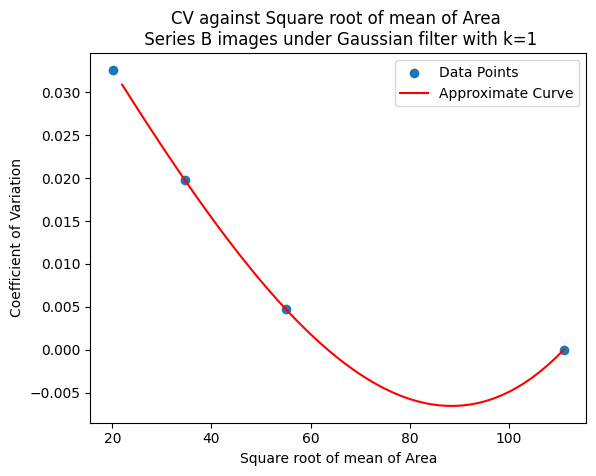
\includegraphics[width=1\linewidth]{Report/Result_Images/series_B_Gaussian_kernel_1_area.png} 
\caption{Image Series B with Gaussian Kernel = 1}
\label{SeriesB-Gaussian-Kernel1-AreaGraph}
\end{center} 
\end{minipage}
\hfill
\vspace{0.2 cm}
\begin{minipage}[h]{0.47\linewidth}
\begin{center}
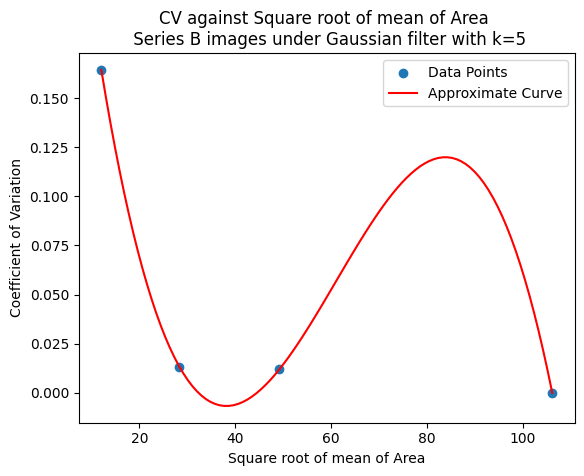
\includegraphics[width=1\linewidth]{Report/Result_Images/series_B_Gaussian_kernel_5_area.png} 
\caption{Image Series B with Gaussian Kernel = 5}
\label{SeriesB-Gaussian-Kernel5-AreaGraph}
\end{center}
\end{minipage}
\vfill
\vspace{0.2 cm}
\begin{minipage}[h]{0.47\linewidth}
\begin{center}
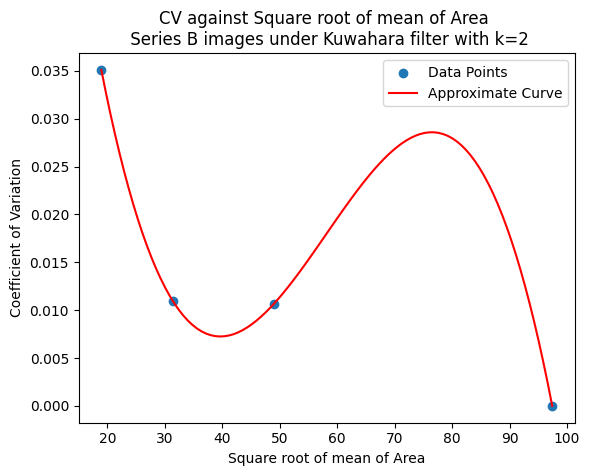
\includegraphics[width=1\linewidth]{Report/Result_Images/series_B_Kuwahara_kernel_2_area.png} 
\caption{Image Series B with Kuwahara Kernel = 2}
\label{SeriesB-Kuwahara-Kernel2-AreaGraph}
\end{center}
\end{minipage}
\hfill
\begin{minipage}[h]{0.47\linewidth}
\begin{center}
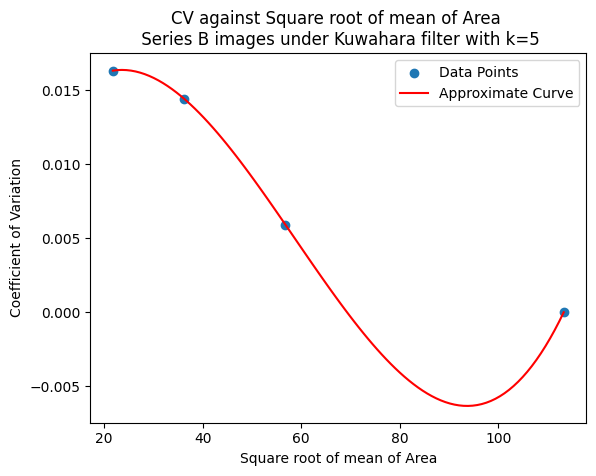
\includegraphics[width=1\linewidth]{Report/Result_Images/series_B_Kuwahara_kernel_5_area.png} 
\caption{Image Series B with Kuwahara Kernel = 5}
\label{SeriesB-Kuwahara-Kernel5-AreaGraph}
\end{center}
\end{minipage}
\caption*{ Graph plotting the relation between coefficient of variation against mean Area for the processed noisy images of series B}
\label{SeriesB-Gaussian/Kuwahara-AreaGraph}
\end{figure}

~\\ Figures \ref{SeriesB-Gaussian-Kernel1-AreaGraph} and \ref{SeriesB-Gaussian-Kernel5-AreaGraph} capture the relationship of square root of area against the coefficient of variation in series B when Gaussian filter is used, while figures \ref{SeriesB-Kuwahara-Kernel2-AreaGraph} and \ref{SeriesB-Kuwahara-Kernel5-AreaGraph} capture the same relationship when Kuwahara Filter is used. 
\par When comparing figures \ref{SeriesB-Gaussian-Kernel1-AreaGraph} and \ref{SeriesB-Gaussian-Kernel5-AreaGraph}, it is evident that the kernel size has a significant effect on the coefficient of variation. We can see this as a smaller kernel size causes the variability to stabilise to a higher value because a smaller neighborhood of pixels is used to calculate the value of the central pixel.  However, with a larger kernel size, the variability initially peaks and then stabilises to a lower value. This is because a larger neighborhood of pixels is used to calculate the central value, reducing the variability in mean intensities. % causes the variability t as the object appears smooth and the area seems to have dropped. As the area has decreased, the mean has also decreased, thus increasing the standard deviation of the image series. This is reflected in the curve, as the curve has plateaued, in \ref{SeriesB-Gaussian-Kernel5-AreaGraph}
\par In Kuwahara filter graphs for series B, figures \ref{SeriesB-Kuwahara-Kernel2-AreaGraph} and \ref{SeriesB-Kuwahara-Kernel5-AreaGraph}, the coefficient of variation has greatly reduced. This is because of the larger kernel size, resulting in a smoother image with much lower variability in pixel intensities.  
\paragraph*{\textbf{Series C}}
\par In the same manner, the following series of graphs plot the relation of the coefficient of variation against the square root of area for the processed noisy images for series C. 
\begin{figure}[h!]
\begin{minipage}[h]{0.47\linewidth}
\begin{center}
\includegraphics[width=1\linewidth]{Report/Result_Images/series_C_Gaussian_kernel_1_area.png} 
\caption{Image Series C with Gaussian Kernel = 1}
\label{SeriesC-Gaussian-Kernel1-AreaGraph}
\end{center} 
\end{minipage}
\hfill
\vspace{0.2 cm}
\begin{minipage}[h]{0.47\linewidth}
\begin{center}
\includegraphics[width=1\linewidth]{Report/Result_Images/series_C_Gaussian_kernel_5_area.png} 
\caption{Image Series C with Gaussian Kernel = 2}
\label{SeriesC-Gaussian-Kernel5-AreaGraph}
\end{center}
\end{minipage}
\vfill
\vspace{0.2 cm}
\begin{minipage}[h]{0.47\linewidth}
\begin{center}
\includegraphics[width=1\linewidth]{Report/Result_Images/series_C_Kuwahara_kernel_2_area.png} 
\caption{Image Series C with Kuwahara Kernel = 2}
\label{SeriesC-Kuwahara-Kernel2-AreaGraph}
\end{center}
\end{minipage}
\hfill
\begin{minipage}[h]{0.47\linewidth}
\begin{center}
\includegraphics[width=1\linewidth]{Report/Result_Images/series_C_Kuwahara_kernel_5_area.png} 
\caption{Image Series C with Kuwahara Kernel = 5}
\label{SeriesC-Kuwahara-Kernel5-AreaGraph}
\end{center}
\end{minipage}
\caption*{Graph plotting the relation between coefficient of variation against mean Area for the processed noisy images of series C}
\label{SeriesC-Gaussian/Kuwahara-AreaGraph}
\end{figure}
\\ Figures \ref{SeriesC-Gaussian-Kernel1-AreaGraph} and \ref{SeriesC-Gaussian-Kernel5-AreaGraph} capture the relationship of square root of area against the coefficient of variation in series C when Gaussian filter is used, while figures \ref{SeriesC-Kuwahara-Kernel2-AreaGraph} and \ref{SeriesC-Kuwahara-Kernel5-AreaGraph} capture the same relationship when Kuwahara Filter is used. 
\par When comparing \ref{SeriesC-Gaussian-Kernel1-AreaGraph} and \ref{SeriesC-Gaussian-Kernel5-AreaGraph}, even though the image series C were already subjected to noise, the processed images produced a higher coefficient of variation when compared to series B. However, the mean area of the objects has greatly reduced when compared to series B. As a result, some of the objects were unrecognizable, as seen in figure \ref{SeriesC-Gaussian-Kernel5-AreaGraph}, only 3 of the 4 images held data that could be processed. 
\par Similarly, in Kuwahara filter graphs for series B, figures \ref{SeriesC-Kuwahara-Kernel2-AreaGraph} and \ref{SeriesC-Kuwahara-Kernel5-AreaGraph}, the coefficient of variation has greatly improved in series C, as it is a edge preserving filter. 
\subsubsection*{Graphs plotting the CV against Square Root of Perimeter}
~\\ In addition to exploring the relationship between the coefficient of variation and square root of area, the relationship between coefficient of variation and square root of perimeter was also explored. This resulted in the following sets of graphs plotting said relation. 
\paragraph*{\textbf{Series B}}
The following series of graphs plot the relation of the coefficient of variation against the square root of perimeter for the processed noisy images for series B. 
\begin{figure}[h!]
\begin{minipage}[h]{0.47\linewidth}
\begin{center}
\includegraphics[width=1\linewidth]{Report/Result_Images/series_B_Gaussian_kernel_1_perimeter.png} 
\caption{Image Series B with Gaussian Kernel = 1}
\label{SeriesB-Gaussian-Kernel1-PerimeterGraph}
\end{center} 
\end{minipage}
\hfill
\vspace{0.2 cm}
\begin{minipage}[h]{0.47\linewidth}
\begin{center}
\includegraphics[width=1\linewidth]{Report/Result_Images/series_B_Gaussian_kernel_5_perimeter.png} 
\caption{Image Series B with Gaussian Kernel = 5}
\label{SeriesB-Gaussian-Kernel5-PerimeterGraph}
\end{center}
\end{minipage}
\vfill
\vspace{0.2 cm}
\begin{minipage}[h]{0.47\linewidth}
\begin{center}
\includegraphics[width=1\linewidth]{Report/Result_Images/series_B_Kuwahara_kernel_2_perimeter.png} 
\caption{Image Series B with Kuwahara Kernel = 2}
\label{SeriesB-Kuwahara-Kernel2-PerimeterGraph}
\end{center}
\end{minipage}
\hfill
\begin{minipage}[h]{0.47\linewidth}
\begin{center}
\includegraphics[width=1\linewidth]{Report/Result_Images/series_B_Kuwahara_kernel_5_perimeter.png} 
\caption{Image Series B with Kuwahara Kernel = 5}
\label{SeriesB-Kuwahara-Kernel5-Perimeter Graph}
\end{center}
\end{minipage}
\caption*{ Graph plotting the relation between coefficient of variation against mean perimeter for the processed noisy images of series B}
\label{SeriesB-Gaussian/Kuwahara-PerimeterGraph}
\end{figure}

~\\ Figures \ref{SeriesB-Gaussian-Kernel1-PerimeterGraph} and \ref{SeriesB-Gaussian-Kernel5-PerimeterGraph} capture the relationship of square root of perimeter against the coefficient of variation in series B when Gaussian filter is used, while figures \ref{SeriesB-Kuwahara-Kernel2-PerimeterGraph} and \ref{SeriesB-Kuwahara-Kernel5-Perimeter Graph} capture the same relationship when Kuwahara Filter is used. 
\par When comparing figures \ref{SeriesB-Gaussian-Kernel1-PerimeterGraph} and \ref{SeriesB-Gaussian-Kernel5-PerimeterGraph}, the CV has increased for the series when kernel size of 5 is used, compared to kernel size 2. This might be because a larger kernel means more smoothing and thus greater blurring of object boundaries. However, it could also mean a shrinkage of object boundarie through a disappearance of the object's contour. This could lead to an overestimation of the perimeter and/or an underestimation of the perimeter of objects, leading to a higher cv. 
\par Similarly, in Kuwahara filter graphs for series B, figures \ref{SeriesB-Kuwahara-Kernel2-PerimeterGraph} and \ref{SeriesB-Kuwahara-Kernel5-Perimeter Graph}, the coefficient of variation has greatly reduced when comparing kernel size 2 and 5.  This is because of the larger kernel size, resulting in a blurred image, which leads to loss in details. 
\newpage
\paragraph*{\textbf{Series C}}
The following series of graphs plot the relation of the coefficient of variation against the square root of perimeter for the processed noisy images for series C. 
\begin{figure}[h!]
\begin{minipage}[h]{0.47\linewidth}
\begin{center}
\includegraphics[width=1\linewidth]{Report/Result_Images/series_C_Gaussian_kernel_1_perimeter.png} 
\caption{Image Series C with Gaussian Kernel = 1}
\label{SeriesC-Gaussian-Kernel1-PerimeterGraph}
\end{center} 
\end{minipage}
\hfill
\vspace{0.2 cm}
\begin{minipage}[h]{0.47\linewidth}
\begin{center}
\includegraphics[width=1\linewidth]{Report/Result_Images/series_C_Gaussian_kernel_5_perimeter.png} 
\caption{Image Series C with Gaussian Kernel = 5}
\label{SeriesC-Gaussian-Kernel5-PerimeterGraph}
\end{center}
\end{minipage}
\vfill
\vspace{0.2 cm}
\begin{minipage}[h]{0.47\linewidth}
\begin{center}
\includegraphics[width=1\linewidth]{Report/Result_Images/series_C_Kuwahara_kernel_2_perimeter.png} 
\caption{Image Series C with Kuwahara Kernel = 2}
\label{SeriesC-Kuwahara-Kernel2-PerimeterGraph}
\end{center}
\end{minipage}
\hfill
\begin{minipage}[h]{0.47\linewidth}
\begin{center}
\includegraphics[width=1\linewidth]{Report/Result_Images/series_C_Kuwahara_kernel_5_perimeter.png} 
\caption{Image Series C with Kuwahara Kernel = 5}
\label{SeriesC-Kuwahara-Kernel5-Perimeter Graph}
\end{center}
\end{minipage}
\caption*{ Graph plotting the relation between coefficient of variation against mean perimeter for the processed noisy images of series C}
\label{SeriesC-Gaussian/Kuwahara-PerimeterGraph}
\end{figure}

~\\ Figures \ref{SeriesC-Gaussian-Kernel1-PerimeterGraph} and \ref{SeriesC-Gaussian-Kernel5-PerimeterGraph} capture the relationship of square root of perimeter against the coefficient of variation in series B when Gaussian filter is used, while figures \ref{SeriesC-Kuwahara-Kernel2-PerimeterGraph} and \ref{SeriesC-Kuwahara-Kernel5-Perimeter Graph} capture the same relationship when Kuwahara Filter is used. 
\par When comparing figures \ref{SeriesC-Gaussian-Kernel1-PerimeterGraph} and \ref{SeriesC-Gaussian-Kernel5-PerimeterGraph}, it is evident that the CV is higher than that of series B. Similar to that of figure \ref{SeriesC-Gaussian-Kernel5-AreaGraph}, only 3 of the 4 images held data that could be processed. This might be due to the noise in Series C. 
\par Similarly, in Kuwahara filter graphs for series C, figures \ref{SeriesC-Kuwahara-Kernel2-PerimeterGraph} and \ref{SeriesC-Kuwahara-Kernel5-Perimeter Graph}, the values show a downward trend with a kernel size of 2, and an upward trend with a kernel size of 5. As discussed in section \textbf{Differences in Area and Perimeter Plot}, this might be because, as the mean perimeter increases, the objects become more homogeneous. 
\newpage

\subsection*{10. Influence of Noise on the Measurements}

\begin{figure}
\includegraphics[width=8cm]{Report/Result_Images/barplot_1.png}
\centering
\caption{Comparison of average area of series of image series B and C}
\label{Area-Comparison-Average}
\end{figure}

\begin{figure}
\includegraphics[width=8cm]{Report/Result_Images/bar_plot_3.png}
\centering
\caption{Comparison of the standard deviation of area of series of image series B and C}
\label{Area-Comparison-Standard Deviation}
\end{figure}

A comparison of the average area of series of images B and C as shown in figure \ref{Area-Comparison-Average} can provide a ton of valuable insight regarding the effect of noise on images. Since the C series is a noisy version of the B series, we can compare and contrast the effect of noise on measurements. As seen in figure \ref{Area-Comparison-Average}, noise tends to reduce the average area of objects in an image. This is because noise in an image tends to obscure the details and features of objects, making their boundaries less distinguishable. Furthermore, noise causes smaller objects to blend into the background and disappear. As a result, the average area of the objects in the image, when measured across multiple instances tends to decrease. \newline

Furthermore, noise tends to increase the entropy and thus increases the standard deviation of the area as shown in figure \ref{Area-Comparison-Standard Deviation}.

\begin{figure}
\includegraphics[width=8cm]{Report/Result_Images/barplot_2.png}
\centering
\caption{Comparison of average perimeter of series of images B and C}
\label{Perimeter-Comparison-Average}
\end{figure}

\begin{figure}
\includegraphics[width=8cm]{Report/Result_Images/bar_plot_4.png}
\centering
\caption{Comparison of the standard deviation of perimeter of series of images B and C}
\label{Perimeter-Comparison-Standard Deviation}
\end{figure}


A comparison of the average perimeter of series of images B and C as shown in figure \ref{Perimeter-Comparison-Average} can provide a ton of valuable insight regarding the effect of noise on images. As seen in figure \ref{Perimeter-Comparison-Average}, noise tends to increase the average perimeter of objects in an image. When noise is present in an image, it can introduce additional edges or boundaries that do not correspond to the actual edges of objects in the scene. These spurious edges can lead to an overestimation of the perimeter of objects because the noise effectively extends the boundaries of objects.
~\\ Furthermore, noise tends to increase the entropy and thus increases the standard deviation of the perimeter as shown in figure \ref{Perimeter-Comparison-Standard Deviation}.
%Denoising algorithms like Gaussian have a blurring effect and tend to smooth over the object intensities by averaging over a neighborhood. However this means that sometimes they may blur the boundaries of an object, causing perceived boundaries to expand and leading to an overestimation of the objects area. This can be seen when comparing the effect of a gaussian filter with kernel 1 and 5 on image B.  They can also have the opposite effect as a smoothing can unintentionally erode the finer contours of an object leading to a shrinkage. This can be seen when comparing the effect of a gaussian filter with kernel 1 and 5 on image C. 
%Denoising algorithms can Gaussian can also decrease the perimeter by smoothing out the boundaries and making much more regular and less jagged, leading to a reduction in fractal behavior and an overall reduction in measurement results. This can be seen by the decrease
\subsection*{11. Plots In Light of The Sampling Theorem}
The Nyquist-Shannon sampling theorem states that in order to accurately reconstruct a signal or an image from its samples, the sampling frequency must be at least twice the maximum frequency present in the signal. This theorem implies that to avoid aliasing (the distortion of the reconstructed image due to undersampling), the sampling frequency (or pixel resolution in this case) must be sufficiently high relative to the features present in the image. \newline
In general we see that  as an application of kernel as the square root of mean of area increases the coefficient of variation decreases. The sampling theorem emphasizes the importance of sufficient sampling frequency to accurately represent the image. In the context of images instead of signals, it implies that capturing more details (using larger kernels) leads to a better representation of the image features, reducing the variability within affected regions and consequently decreasing the coefficient of variation. \newline
In general we see that  as an application of kernel as the square root of mean of perimeter increases the coefficient of variation tends to reach a maximum and then stabilises to a lower value. This suggests that initially, increasing the kernel size leads to capturing more details and hence increased variability and a positive change in the coefficient of variation. However, beyond a certain point, capturing finer details becomes less significant, and the variability stabilizes or decreases.


\newpage

\section*{Part 2.4}
Signal to Noise Ration (SNR or S/N) is an important aspect in image processing, which indicates the quality of the image. 

The SNR is expressed as, 
\begin{equation*}
    SNR = \mu/\sigma'
\end{equation*}
where $\mu$ is the average 
and $\sigma$ is the standard deviation. 
The higher the SNR, the better the image (as it typically means that the image has better signal/quality than the noise in the image). \subsection*{12. SNRs of the Images}

The following table contain the SNRs of the original image series - Series A, Series B and Series C

\begin{table}[h!]
\centering
\begin{tabular}{|c|c|c|c|c|}
\hline
\textbf{} & \textbf{Series A} & \textbf{Series B} & \textbf{Series C}\\ \hline
rect 1 & 3.28 & 2.65 &  2.16 \\ \hline
rect 2 & 2.63 & 2.30  & 2.04 \\ \hline
rect 3 & 3.63 & 2.82  &  2.19 \\ \hline
rect 4 & 5.45 & 3.42  & 2.32\\ \hline
\end{tabular}
\caption{Table of the SNRs of the original image series - A, B, C}
\label{tab:SNR-original}
\end{table}
~\\ Since the image series A is devoid of noise, we can see that the SNR is very high for those. In Image series B and C, the SNRs are gradually lower due to the noise in the images. 
~\\The following table [table \ref{tab:SNR of processed image series B}] contain the SNRs of the processed images with Gaussian and Kuwahara Filters for image series B, with the SNRs of the unprocessed image series in the first column for reference.

\begin{table}[h!]
\setlength{\heavyrulewidth}{1.5pt}
\setlength{\abovetopsep}{4pt}
\centering
\caption{Table containing the SNRs of the processed noisy image series B}
\begin{adjustbox}{width=0.5\textwidth,center=\textwidth}
\begin{tabular}{*6c} % Your table content here
\toprule
Image & Original SNR & \multicolumn{2}{c}{Gaussian} & \multicolumn{2}{c}{Kuwahara}\\
\midrule
{}   & {} & 1   & 5    & 2   & 5\\
1b   & 2.65 & 3.63 & 3.97   & 2.65  & 3.44\\
2b   & 2.30  &  3.01 & 3.53   & 2.30  & 2.80\\
3b   & 2.82  & 4.08  &  5.08   & 2.82  & 3.83\\
4b   & 3.42  & 5.93  &  8.58   & 3.42  & 5.58\\
\bottomrule
\end{tabular}
\label{tab:SNR of processed image series B}
\end{adjustbox}
\end{table}
~\\ When comparing the original SNRs of the image to the SNRs of the processed images, there is a significant improvement. The SNRs are progressively better with the increase in kernel size. Both Gaussian and Kuwahara filter has processed the image comparably well, as the SNRs are similar, if not higher to the original image.
\newpage
The following table [table \ref{tab:SNR of processed image series C}] contain the SNRs of the processed images with Gaussian and Kuwahara Filters for image series C, for image series B, with the SNRs of the unprocessed image series in the first column for reference.
\begin{table}[h!]
\setlength{\heavyrulewidth}{1.5pt}
\setlength{\abovetopsep}{4pt}
\centering
\caption{Table containing the SNRs of the processed noisy image series C}
\begin{adjustbox}{width=0.5\textwidth,center=\textwidth}
\begin{tabular}{*6c} % Your table content here
\toprule
Image & Original SNR & \multicolumn{2}{c}{Gaussian} & \multicolumn{2}{c}{Kuwahara}\\
\midrule
{}   & {} & 1   & 5    & 2   & 5\\
1c   & 2.16 & 5.22 & 7.08   & 2.16  & 4.78\\
2c   & 2.04  & 4.58 & 6.37  & 2.04  & 4.05\\
3c   & 2.19 & 5.54  &  8.87   & 2.19 & 5.11\\
4c   & 2.32 & 6.75  &  14.30   & 2.32  & 6.71\\
\bottomrule
\end{tabular}
\label{tab:SNR of processed image series C}
\end{adjustbox}
\end{table}
\subsection*{13. Relation of SNRs to the measurements}

\paragraph*{\textbf{Series B}}
The following series of graphs plot the relation of the log of the measurements against the signal to noise ratio for the images for series B. 

~\\Figures \ref{SeriesB_Log_Gaussian_1} and \ref{SeriesB_Log_Gaussian_5} plot the relationship of the log of measurements against SNR when Gaussian filter is used (for kernel sizes 1 and 5), and figures \ref{SeriesB_Log_Kuwahara_2} and \ref{SeriesB_Log_Kuwahara_5} plot said relationship when Kuwahara filter is used (for kernel sizes 2 and 5).
\begin{figure}[h!]
\begin{minipage}[h]{0.47\linewidth}
\begin{center}
\includegraphics[width=1\linewidth]{Report/Result_Images/log_seriesB_Gaussian_1.png} 
\caption{Image Series B with Gaussian Kernel = 1}
\label{SeriesB_Log_Gaussian_1}
\end{center} 
\end{minipage}
\hfill
\vspace{0.2 cm}
\begin{minipage}[h]{0.47\linewidth}
\begin{center}
\includegraphics[width=1\linewidth]{Report/Result_Images/log_seriesB_Gaussian_5.png} 
\caption{Image Series B with Gaussian Kernel = 5}
\label{SeriesB_Log_Gaussian_5}
\end{center}
\end{minipage}
\vfill
\vspace{0.2 cm}
\begin{minipage}[h]{0.47\linewidth}
\begin{center}
\includegraphics[width=1\linewidth]{Report/Result_Images/log_seriesB_Kuwahara_2.png} 
\caption{Image Series B with Kuwahara Kernel = 2}
\label{SeriesB_Log_Kuwahara_2}
\end{center}
\end{minipage}
\hfill
\begin{minipage}[h]{0.47\linewidth}
\begin{center}
\includegraphics[width=1\linewidth]{Report/Result_Images/log_seriesB_Kuwahara_5.png} 
\caption{Image Series B with Kuwahara Kernel = 5}
\label{SeriesB_Log_Kuwahara_5}
\end{center}
\end{minipage}
\caption*{ Graph plotting the relation between log of measurements against Signal to Noise Ratio for the processed noisy images of series C}
\label{SeriesB_Log_SNR}
\end{figure}
\newpage
\paragraph*{\textbf{Series C}}
The following series of graphs plot the relation of the log of the measurements against the signal to noise ratio for the images for series C. 
~\\Figures \ref{SeriesC_Log_Gaussian_1} and \ref{SeriesC_Log_Gaussian_5} plot the relationship of the log of measurements against SNR when Gaussian filter is used (for kernel sizes 1 and 5), and figures \ref{SeriesC_Log_Kuwahara_2} and \ref{SeriesC_Log_Kuwahara_5} plot said relationship when Kuwahara filter is used (for kernel sizes 2 and 5).
\begin{figure}[h!]
\begin{minipage}[h]{0.47\linewidth}
\begin{center}
\includegraphics[width=1\linewidth]{Report/Result_Images/log_seriesC_Gaussian_1.png} 
\caption{Image Series C with Gaussian Kernel = 1}
\label{SeriesC_Log_Gaussian_1}
\end{center} 
\end{minipage}
\hfill
\vspace{0.2 cm}
\begin{minipage}[h]{0.47\linewidth}
\begin{center}
\includegraphics[width=1\linewidth]{Report/Result_Images/log_seriesC_Gaussian_5.png} 
\caption{Image Series C with Gaussian Kernel = 5}
\label{SeriesC_Log_Gaussian_5}
\end{center}
\end{minipage}
\vfill
\vspace{0.2 cm}
\begin{minipage}[h]{0.47\linewidth}
\begin{center}
\includegraphics[width=1\linewidth]{Report/Result_Images/log_seriesC_Kuwahara_2.png} 
\caption{Image Series C with Kuwahara Kernel = 2}
\label{SeriesC_Log_Kuwahara_2}
\end{center}
\end{minipage}
\hfill
\begin{minipage}[h]{0.47\linewidth}
\begin{center}
\includegraphics[width=1\linewidth]{Report/Result_Images/log_seriesC_Kuwahara_5.png} 
\caption{Image Series B with Kuwahara Kernel = 5}
\label{SeriesC_Log_Kuwahara_5}
\end{center}
\end{minipage}
\caption*{ Graph plotting the relation between log of measurements against Signal to Noise Ratio for the processed noisy images of series C}
\label{SeriesC_Log_SNR}
\end{figure}
\paragraph*{\textbf{Observations}}
~\\ A decreasing SNR as the logarithm of the measurement increases indicates that as the measurement value grows, it becomes increasingly challenging to distinguish the signal from the background noise.
\par This could be due to various factors such as limitations in the measurement system itself, environmental noise, or intrinsic noise in the signal itself. Our understanding is that as smoothing occurs measurements like area and perimeter increase (corresponding to an increase in size of object) and simultaneously noise is reduced. However, in some cases the signal is also oversuppressed leading to an overall lower signal-to-noise ratio.

\newpage
\appendix
\textbf{Appendix}
\section{Code}
%\lstinputlisting {ImageAnalysisPractical2.ipynb}
%\uselist
%\begin{lgrind}
%   \input ImageAnalyisPractical2.ipynb
%\end{lgrind}

%\lstinputlisting[language=Python]{ImageAnalysisPractical2.ipynb}
%\lstinputlisting{ImageAnalysisPractical2.ipyb}

\end{document}


% ---- Bibliography ----
%
% BibTeX users should specify bibliography style 'splncs04'.
% References will then be sorted and formatted in the correct style.
%
% \bibliographystyle{splncs04}
% \bibliography{mybibliography}
%
% \begin{thebibliography}{8}
% \bibitem{ref_article1}
% Author, F.: Article title. Journal \textbf{2}(5), 99--110 (2016)

% \bibitem{ref_lncs1}
% Author, F., Author, S.: Title of a proceedings paper. In: Editor,
% F., Editor, S. (eds.) CONFERENCE 2016, LNCS, vol. 9999, pp. 1--13.
% Springer, Heidelberg (2016). \doi{10.10007/1234567890}

% \bibitem{ref_book1}
% Author, F., Author, S., Author, T.: Book title. 2nd edn. Publisher,
% Location (1999)

% \bibitem{ref_proc1}
% Author, A.-B.: Contribution title. In: 9th International Proceedings
% on Proceedings, pp. 1--2. Publisher, Location (2010)

% \bibitem{ref_url1}
% LNCS Homepage, \url{http://www.springer.com/lncs}, last accessed 2023/10/25
% \end{thebibliography}
\end{document}